\section{Model Details}
\label{app:model}

\paragraph{Streams.} The encoder gives
\begin{equation}
\bm{A}=\mathrm{Enc}(\bm{x})=[\bm{a}_1;\dots;\bm{a}_N]\in\R^{N\times d},
\label{eq:enc}
\end{equation}
row $\bm{a}_i$ describing about 80\,ms centred at $\bar{t}_i=(i-\tfrac12)T/N$. The diarizer (chunks of 0.72\,s, 0.32\,s right
context, a speaker cache) gives
\begin{equation}
\bm{P}=\mathrm{Diar}(\bm{x})\in[0,1]^{F\times S},\quad F=\lceil T/0.08\,\mathrm{s}\rceil,
\label{eq:diar}
\end{equation}
resampled linearly in time to the token centres,
\begin{equation}
\tilde{\bm{P}}=\mathrm{Interp}(\bm{P};\,\bar{t}_1,\dots,\bar{t}_N)\in[0,1]^{N\times S}.
\label{eq:interp}
\end{equation}
With $\tilde{\bm{P}}$ zero-padded to $MK$ rows, $M=\lceil N/K\rceil$, the projector computes
\begin{equation}
\bm{z}_j=\sum_{r=1}^{K}\bm{W}^{(r)}\,\tilde{\bm{p}}_{(j-1)K+r}+\bm{b}\in\R^{h},
\label{eq:conv}
\end{equation}
\begin{equation}
\bm{s}_j=\bm{W}_2\,\mathrm{GELU}\big(\bm{W}_1\mathrm{GELU}(\bm{z}_j)+\bm{b}_1\big)+\bm{b}_2\in\R^{d},
\label{eq:mlp}
\end{equation}
with $h=1024$; $\bm{W}_2,\bm{b}_2$ start at zero, so training starts from the pretrained Thinker reading zero vectors and
phases the speaker stream in only as far as it lowers the loss. The Thinker defines
\begin{equation}
p_\theta(\bm{y}\mid\bm{x})=\prod_{u=1}^{|\bm{y}|}p_\theta\big(y_u\mid \bm{y}_{<u},\bm{E},\bm{\iota}\big).
\label{eq:ar}
\end{equation}

\paragraph{Slot-consistent targets.} Per meeting, reference speakers $\rho\in\mathcal{R}$ are mapped to slots by
\begin{equation}
\sigma^\star=\arg\max_{\sigma}\sum_{\rho\in\mathcal{R}}\sum_{f=1}^{F_\text{m}}
G_{f,\rho}\,\mathds{1}\big[P_{f,\sigma(\rho)}>0.5\big],
\label{eq:slotmap}
\end{equation}
over injective maps $\sigma$, with $G_{f,\rho}\in\{0,1\}$ marking reference speech of $\rho$ in frame $f$ of the meeting;
an utterance by $\rho$ is labelled $\sigma^\star(\rho)$. Rounding can make $\alpha_n=\beta_n$ for very short segments
(\num{v6:sameb:en2zh:O2}\% of \sys{}'s En$\rightarrow$Zh segments); such a segment keeps its text but counts as
zero-length speech in DER. By design, hesitations have no target segment.

\paragraph{Deadline timing.} An utterance's reference translation is split at punctuation into chunks $c_1,\dots,c_J$;
chunk $j$ covers the fraction
\begin{equation}
\phi_j=\textstyle\sum_{j'\le j}|c_{j'}|\,/\,\sum_{j'=1}^{J}|c_{j'}|
\label{eq:frac}
\end{equation}
of the utterance and ends at $e_j=\mathrm{end}(w_{\lceil\phi_j|\bm{w}|\rceil})$ for the time-aligned source words
$\bm{w}$, or at $e_j=a+\phi_j(b-a)$ where no word timings exist (the re-voiced Chinese source). The target of read $r$ is
\begin{equation}
\bm{y}^{(r)}=\Big(\mathop{\Vert}_{j:\,r(j)=r}\big[\spk{k_j}\,\tim{\alpha_j}\,c_j\,\tim{\beta_j}\big]\Big)\,\Vert\,\eta_r .
\label{eq:readtarget}
\end{equation}

\paragraph{Voices and playback layout.} Slot $k$'s solo frames are
\begin{equation}
m_{f,k}=\mathds{1}\big[P_{f,k}>0.5\big]\prod_{k'\neq k}\mathds{1}\big[P_{f,k'}<0.5\big].
\label{eq:alone}
\end{equation}
Within a speaker's stream, segment $n$ of duration $D_n$ starts at
\begin{equation}
\pi_n=\max\big(\zeta_n,\;\pi_{n-1}+D_{n-1}\big),
\label{eq:layout}
\end{equation}
with $\zeta_n$ its release time (the source start offline). The single-channel layout (Appendix~\ref{app:v9proto})
serialises all streams of a meeting, $\pi_n=\max(\zeta_n,\pi_{n-1}+D_{n-1}+g\,\mathds{1}[k_n\neq k_{n-1}])$ with
$g=0.2$\,s between speakers.

\section{Data Construction}
\label{app:data}

\begin{table}[t]
\centering\small
\resizebox{\columnwidth}{!}{\begin{tabular}{lrrrrrrr}
\toprule
Split & Mtg. & Windows & Hours & Mean\,s & Utt. & Multi\,\% & Ovl.\,\% \\
\midrule
\multicolumn{8}{l}{\emph{En$\rightarrow$Zh}} \\
Train & 137 & 21{,}581 & 36.8 & 6.1 & 54{,}824 & 38.5 & 38.2 \\
Dev & 18 & 3{,}203 & 5.2 & 5.9 & 8{,}206 & 40.0 & 39.6 \\
Test & 16 & 2{,}375 & 3.9 & 5.9 & 5{,}790 & 35.0 & 34.7 \\
\multicolumn{8}{l}{\emph{Zh$\rightarrow$En}} \\
Train & 127 & 27{,}953 & 48.5 & 6.3 & 69{,}540 & 37.4 & 34.6 \\
Dev & 15 & 3{,}366 & 5.7 & 6.1 & 8{,}340 & 39.3 & 36.6 \\
Test & 16 & 3{,}317 & 5.8 & 6.3 & 8{,}634 & 36.5 & 34.5 \\
\multicolumn{8}{l}{\emph{Zh$\rightarrow$En, AliMeeting (real meetings)}} \\
Test & 20 & 4{,}243 & 7.5 & 6.4 & 9{,}730 & 33.4 & 33.2 \\
\bottomrule
\end{tabular}}
\caption{Reference windows of the two directions. En$\rightarrow$Zh: AMI IHM-mix with Chinese references;
Zh$\rightarrow$En: the re-voiced Chinese meetings (Appendix~\ref{app:zhdata}) with the AMI English transcripts as
references. \emph{Multi}: windows with two or more speakers; \emph{Ovl.}: windows in which two utterances overlap.}
\label{tab:data}
\end{table}


\paragraph{Translations.} Every AMI utterance (IHM segmentation, official train/dev/test meetings) is translated by
three MT systems (Hy-MT2-30B-A3B, NiuTrans LMT-60-4B and MiLMMT-46-4B). One candidate is selected with reference-free
quality estimation (XCOMET-XL~\citep{guerreiro2024xcomet} and an XLM-R-XL estimator) and the chrF agreement between candidates. The selected
translation is also synthesised in the speaker's voice (VoxCPM2), and the synthesis is checked for audibility and
intelligibility (Whisper large-v3 CER). Of the 12{,}643 test utterances, 96.3\% received a translation and speech.

\paragraph{Review.} A window enters our data only if all its non-hesitation utterances have a non-empty translation
whose speech decodes and is not silent. A stricter review also requires the speech not to be over-long and to be
recognised with CER $\le0.3$; it rejects many windows with short back-channels and is used only as a test subset
(1{,}454 of 2{,}375 test windows).

\paragraph{Windows.} Reference windows are AMI utterance groups: utterances that overlap or touch are grouped, and a
group longer than 20\,s is dropped. Diarizer windows (training only) open at the first active diarizer frame and close
after 1\,s without activity or at 20\,s; they are padded by 0.2\,s before and 0.3\,s after. A window is dropped if an
utterance overlapping it has less than 90\% of its duration inside the window.

\section{Instruction}
\label{app:prompt}

The instruction $\bm{\iota}$ is the Thinker's speech translation instruction followed by: \emph{``Several people are
speaking. For every utterance write \texttt{<|spk k|><|t a|>}translation\texttt{<|t b|>}: k is the speaker's slot in the
speaker stream, a and b are its start and end in 80 ms steps from the start of the audio, utterances in order of
start.''} The prompted baseline receives the same audio without speaker tokens and the plain translation
instruction.

\section{Metrics}
\label{app:metrics}

\paragraph{cpBLEU.} Let meeting $m$ consist of windows $\mathcal{W}_m$. For output slot $k$ and window $w$, let
$H_{w,k}$ be the concatenated text of all segments with label $k$, and for reference speaker $\rho$ let $G_{w,\rho}$ be
the concatenated reference translations of $\rho$ in $w$. The session-level matching is
\begin{equation}
\pi_m=\arg\max_{\pi}\sum_{k}\mathrm{chrF}\big(H_{m,k},\,G_{m,\pi(k)}\big),
\end{equation}
where $H_{m,k}=\Vert_{w\in\mathcal{W}_m}H_{w,k}$ and $G_{m,\rho}=\Vert_{w\in\mathcal{W}_m}G_{w,\rho}$ are the
meeting-level concatenations and $\pi$ ranges over one-to-one partial maps from output slots to reference speakers. cpBLEU$_\text{sess}$ is corpus BLEU over the
pairs $(H_{w,k},G_{w,\pi_m(k)})$ of all windows and matched slots, plus $(H_{w,k},\varnothing)$ for unmatched output
slots and $(\varnothing,G_{w,\rho})$ for unmatched reference speakers; missing or extra speakers are therefore
penalised through brevity and precision. cpBLEU$_\text{win}$ uses a separate matching $\pi_w$ for every window.

\paragraph{DER.} Output segments $(k_n,a_n,b_n)$ and reference utterances (hesitations excluded) are rasterised on
10\,ms frames; output labels are mapped to reference speakers per meeting by maximal total overlap (Hungarian), and
missed speech, false alarm and confusion are summed over all windows without a collar.

\paragraph{LAAL.} For a window of duration $T$ whose committed output has $|\hat{\bm{y}}|$ characters with commit times
$d_1\le\dots\le d_{|\hat{\bm{y}}|}$ and whose reference has $|\bm{y}^\star|$ characters,
\begin{equation}
\mathrm{LAAL}=\frac{1}{i^\ast}\sum_{i=1}^{i^\ast}\Big(d_i-(i-1)\frac{T}{\max(|\hat{\bm{y}}|,|\bm{y}^\star|)}\Big),
\end{equation}
where $i^\ast$ is the index of the first character committed at or after $T$ (or $|\hat{\bm{y}}|$). We average LAAL
over windows.

\paragraph{tcpBLEU.} Whole meetings have no windows to pair output with reference, so we score time-constrained:
(1) reference units are a speaker's scored utterances chained while less than 1\,s apart (a model may write two
consecutive utterances of one person as one segment); (2) output slots are matched to speakers per meeting by chrF over
the whole meeting's text, as for cpBLEU; (3) each output segment, on the meeting clock and widened by a collar $c$ on both
sides, goes to the annotated utterance it overlaps most: if that utterance was not scored (a hesitation, or speech the
reference windows dropped) the segment is ignored; if it belongs to the segment's matched speaker the segment joins that
utterance's unit; otherwise it joins the matched speaker's own unit that it overlaps most, and if there is none it is an
insertion. A segment spanning two units counts once, for the one it overlaps most; several segments in one unit are
joined in time order; a segment overlapping no annotated speech is an insertion. tcpBLEU is corpus BLEU over
(unit hypothesis, unit reference) pairs plus (insertion, empty) pairs. \emph{Example}: speakers A and B, A says $u_1$
(0--4\,s) and $u_2$ (4.5--8\,s), B says ``yes'' (2--2.5\,s) inside $u_1$ and $u_3$ (6--9\,s) overlapping $u_2$. A's units:
$\{u_1u_2\}$ (0.5\,s apart); B's: $\{\text{yes}\}$, $\{u_3\}$. An output segment of A over 0--8\,s goes to A's unit; an
output ``yes'' labelled A at 2--2.5\,s overlaps $u_1$ most, belongs to A's unit, and is therefore scored there (a wrong
attribution costs B's ``yes'' as a deletion and adds an extra word to A's unit); an output of B at 6--9\,s goes to
$u_3$; an output at 10--11\,s with no speech is an insertion. Table~\ref{tab:collar} varies $c$.

\begin{table}[h]
\centering\small
\setlength{\tabcolsep}{3pt}
\resizebox{\ifdim\width>\columnwidth\columnwidth\else\width\fi}{!}{\begin{tabular}{lllrrrr}
\toprule
Set & System & Run & 0\,s & 0.5\,s & 1\,s & 2\,s \\
\midrule
En$\rightarrow$Zh & Simul & windows & 42.45 & 42.39 & 42.34 & 42.15 \\
En$\rightarrow$Zh & Simul & online & 39.40 & 39.36 & 39.29 & 38.85 \\
En$\rightarrow$Zh & LA2 & windows & 27.64 & 27.64 & 27.64 & 27.45 \\
En$\rightarrow$Zh & LA2 & online & 33.74 & 33.82 & 33.78 & 33.43 \\
Zh$\rightarrow$En & Simul & windows & 25.39 & 25.32 & 25.30 & 25.07 \\
Zh$\rightarrow$En & Simul & online & 25.19 & 25.16 & 25.11 & 24.91 \\
Zh$\rightarrow$En & LA2 & windows & 24.73 & 24.73 & 24.69 & 24.46 \\
Zh$\rightarrow$En & LA2 & online & 24.41 & 24.38 & 24.34 & 24.11 \\
AliMeeting & Simul & windows & 12.05 & 12.03 & 12.02 & 11.97 \\
AliMeeting & Simul & online & 11.65 & 11.63 & 11.62 & 11.55 \\
AliMeeting & LA2 & windows & 11.73 & 11.72 & 11.73 & 11.69 \\
AliMeeting & LA2 & online & 10.09 & 10.11 & 10.11 & 10.05 \\
\bottomrule
\end{tabular}}
\caption{tcpBLEU on the whole-meeting subset at four collars (Simul: \sys{}-Simul; LA2: \sys{} + LA2; windows: the reference-window run of the same system, scored on the same meetings).}
\label{tab:collar}
\end{table}


\section{Hyperparameters}
\label{app:hyper}

\paragraph{Simul training rows.} Reads with nothing due are kept with probability 0.5; whole-window (20\%) and
single-speaker (15\%) rows are mixed in.

\begin{table}[h]
\centering\small
\setlength{\tabcolsep}{3pt}
\resizebox{\columnwidth}{!}{\begin{tabular}{lcc}
\toprule
 & \sys{} (offline) & \sys{}-Simul \\
\midrule
Initialisation & Qwen3-Omni Thinker & \sys{} (offline), merged \\
Directions & both & one model each \\
Diarizer preset & offline & low latency (1.04\,s) \\
Rows & 67{,}795 & 128{,}879 / 160{,}957 \\
Steps & 2{,}000 & 3{,}000 \\
GPUs (H200) & 8 & 8 \\
Batch (global / micro) & 64 / 8 & 64 / 8 \\
Learning rate & \multicolumn{2}{c}{$10^{-4}\to10^{-5}$, cosine, 50 warm-up} \\
LoRA & \multicolumn{2}{c}{$r=32$, $\alpha=64$, q/k/v/o, 48 layers} \\
Loss weights $\omega$ & \multicolumn{2}{c}{speaker 2, time 1.5, other 1} \\
Posterior perturbation & \multicolumn{2}{c}{$p=0.2$, $\mathcal{N}(0,0.1^2)$, shift $\le1$ frame} \\
Single-speaker rows & 15\% & 15\% (+20\% offline) \\
Read interval / lag & -- & $\Delta=1$\,s (-M: 0.5/1/2\,s) / $\epsilon=1$\,s \\
\bottomrule
\end{tabular}}
\caption{Training hyperparameters (\sys{}-Simul: En$\rightarrow$Zh / Zh$\rightarrow$En).}
\label{tab:hyper}
\end{table}

\section{Latency and Full Metrics}
\label{app:full}

\begin{figure*}[t]
\centering
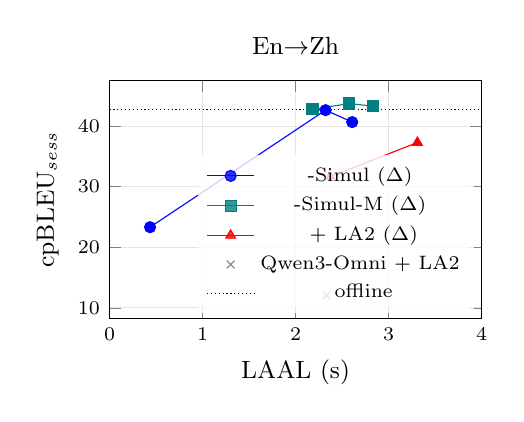
\begin{tikzpicture}\begin{axis}[width=0.52\textwidth, height=4.6cm, xlabel={LAAL (s)}, ylabel={cpBLEU$_\text{sess}$}, title={En$\rightarrow$Zh}, title style={font=\small}, tick label style={font=\scriptsize}, label style={font=\small}, xmin=0, xmax=4, enlarge y limits=0.12, grid=major, grid style={gray!20}, legend style={font=\scriptsize, at={(0.98,0.02)}, anchor=south east, draw=none, fill=white, fill opacity=0.8, text opacity=1}]
\addplot[blue, mark=*] coordinates {(0.435,23.31) (2.323,42.63) (2.609,40.66)}; \addlegendentry{\sys{}-Simul ($\Delta$)}
\addplot[teal, mark=square*] coordinates {(2.183,42.79) (2.579,43.72) (2.832,43.29)}; \addlegendentry{\sys{}-Simul-M ($\Delta$)}
\addplot[red, mark=triangle*] coordinates {(2.373,31.64) (3.310,37.29)}; \addlegendentry{\sys{} + LA2 ($\Delta$)}
\addplot[gray, only marks, mark=x] coordinates {(2.333,12.07)}; \addlegendentry{Qwen3-Omni + LA2}
\addplot[black, densely dotted, domain=0:4, samples=2] {42.81}; \addlegendentry{\sys{} offline}
\end{axis}\end{tikzpicture}
\hfill
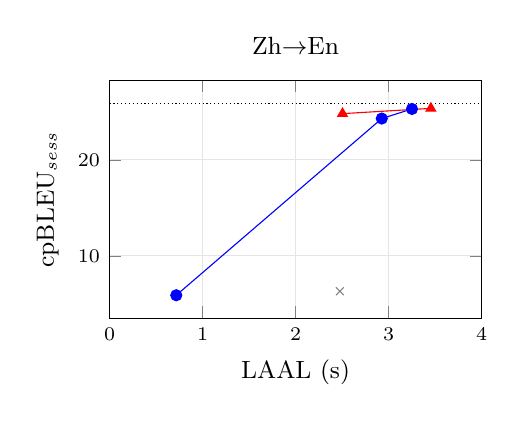
\begin{tikzpicture}\begin{axis}[width=0.52\textwidth, height=4.6cm, xlabel={LAAL (s)}, ylabel={cpBLEU$_\text{sess}$}, title={Zh$\rightarrow$En}, title style={font=\small}, tick label style={font=\scriptsize}, label style={font=\small}, xmin=0, xmax=4, enlarge y limits=0.12, grid=major, grid style={gray!20}]
\addplot[blue, mark=*] coordinates {(0.717,5.89) (2.927,24.30) (3.252,25.30)};
\addplot[red, mark=triangle*] coordinates {(2.505,24.81) (3.455,25.36)};
\addplot[gray, only marks, mark=x] coordinates {(2.476,6.31)};
\addplot[black, densely dotted, domain=0:4, samples=2] {25.86};
\end{axis}\end{tikzpicture}
\caption{Latency--quality trade-off (text) over the read interval $\Delta\in\{0.5,1,2\}$\,s (left to right).
\sys{}-Simul is trained at $\Delta=1$\,s, \sys{}-Simul-M at mixed intervals (En$\rightarrow$Zh). The dotted line is the offline \sys{}. Numbers in Table~\ref{tab:tradeoff}.}
\label{fig:tradeoff}
\end{figure*}

\begin{table}[t]
\centering\small
\setlength{\tabcolsep}{2.6pt}
\resizebox{\columnwidth}{!}{\begin{tabular}{lccccc}
\toprule
System & LAAL\,s & cpBLEU$_\text{sess}$ & BLEU$_\text{blind}$ & Spk & DER \\
\midrule
Cascade, same-data translator & -- & 15.25 & 15.58 & 92.5 & 13.1 \\
Cascade, turn-trained translator & -- & 13.05 & 13.11 & 76.4 & 26.0 \\
\sys{} w/o speaker stream & -- & 8.34 & 16.38 & 87.1 & 52.0 \\
\quad + diarizer relabelling & -- & 15.99 & 16.38 & 86.8 & 12.9 \\
\sys{} (offline) & -- & 14.90 & 15.11 & 91.9 & 14.7 \\
\midrule
\sys{} (offline) + LA2 & 2.84 & 12.10 & 12.55 & 91.7 & 12.9 \\
\sys{}-Simul model + LA2 & 3.40 & 13.44 & 13.62 & 91.3 & 10.6 \\
\sys{}-Simul & 3.62 & 11.98$\pm$1.41$^{2}$ & 12.14 & 91.5 & 10.8 \\
\bottomrule
\end{tabular}}
\caption{Real Mandarin meetings (AliMeeting test, Zh$\rightarrow$En, 20 meetings, 4{,}243 reference windows; zero-shot: no AliMeeting data in training). The English references are machine translations of the human transcripts (their automatic quality estimate: Appendix~\ref{app:qe7}).}
\label{tab:real7}
\end{table}

\begin{table}[t]
\centering\small
\setlength{\tabcolsep}{3pt}
\resizebox{\columnwidth}{!}{\begin{tabular}{llccccc}
\toprule
Set & Seed & cpBLEU$_\text{sess}$ & cpBLEU$_\text{win}$ & LAAL\,s & Spk & Empty \\
\midrule
En$\rightarrow$Zh & 1 & 42.63 & 43.06 & 2.32 & 90.6 & 0.0 \\
 & 2 & 43.10 & 43.57 & 2.35 & 90.4 & 0.0 \\
 & 3 & 43.52 & 44.01 & 2.53 & 90.3 & 0.0 \\
 & mean $\pm$ s.d. & 43.08 $\pm$ 0.45 & & 2.40 & & \\
\midrule
Zh$\rightarrow$En & 1 & 24.30 & 25.81 & 2.93 & 93.2 & 0.0 \\
 & 2 & 22.79 & 24.07 & 3.16 & 93.0 & 0.0 \\
 & mean $\pm$ s.d. & 23.55 $\pm$ 1.07 & & 3.04 & & \\
\midrule
AliMeeting & 1 & 12.97 & 13.09 & 3.09 & 91.5 & 0.0 \\
 & 2 & 10.98 & 11.08 & 4.15 & 91.5 & 0.0 \\
 & mean $\pm$ s.d. & 11.98 $\pm$ 1.41 & & 3.62 & & \\
\bottomrule
\end{tabular}}
\caption{\sys{}-Simul per training seed ($\Delta{=}1$\,s, reference windows; AliMeeting uses the Zh$\rightarrow$En models). Seeds differ only in the random seed (seed 3 of En$\rightarrow$Zh was retrained from scratch after a resume had restarted its learning-rate schedule). Empty: windows with no output (failures).}
\label{tab:seeds7}
\end{table}


\paragraph{Read interval.} Varying $\Delta$ at test time (Figure~\ref{fig:tradeoff}): at 2\,s, \sys{}-Simul loses
\num{cost:en2zh:d2} points for \num{lat:en2zh:d2}\,s more LAAL (LocalAgreement trails by \num{gain:en2zh:simul2}); at
0.5\,s, earlier than any training read, it commits guesses and collapses (\num{tx:en2zh:S2dl_d0.5:cp};
Zh$\rightarrow$En \num{tx:zh2en:S2dl_d0.5:cp}). Drawing the
interval per training window from $\{0.5,1,2\}$\,s (\sys{}-Simul-M) removes the collapse: \num{tx:en2zh:S2dlm_d0.5:cp}
at 0.5\,s with \num{tx:en2zh:S2dlm_d0.5:laal}\,s LAAL, by waiting longer, not by sub-second commits.


\begin{table*}[t]
\centering\small
\setlength{\tabcolsep}{4pt}
\resizebox{\textwidth}{!}{\begin{tabular}{lccccc@{\hskip 10pt}ccccc}
\toprule
 & \multicolumn{5}{c}{En$\rightarrow$Zh} & \multicolumn{5}{c}{Zh$\rightarrow$En} \\
\cmidrule(lr){2-6}\cmidrule(lr){7-11}
System & LAAL & First & cpBLEU$_\text{sess}$ & BLEU$_\text{blind}$ & Len & LAAL & First & cpBLEU$_\text{sess}$ & BLEU$_\text{blind}$ & Len \\
\midrule
Qwen3-Omni + LA2, $\Delta{=}1$\,s & 2.33 & 1.85 & 12.07 & 26.87 & 0.75 & 2.48 & 2.08 & 6.31 & 14.11 & 0.78 \\
\sys{} (offline) + LA2, $\Delta{=}1$\,s & 2.37 & 2.23 & 31.64 & 32.74 & 1.18 & 2.50 & 2.24 & 24.81 & 27.67 & 0.94 \\
\sys{} (offline) + LA2, $\Delta{=}2$\,s & 3.31 & 2.98 & 37.29 & 38.33 & 1.06 & 3.46 & 2.98 & 25.36 & 28.21 & 0.94 \\
\sys{}-Simul, $\Delta{=}0.5$\,s & 0.43 & 0.25 & 23.31 & 24.30 & 1.27 & 0.72 & 0.24 & 5.89 & 10.79 & 1.34 \\
\sys{}-Simul, $\Delta{=}1$\,s & 2.32 & 2.19 & 42.63 & 42.80 & 0.99 & 2.93 & 2.79 & 24.30 & 26.71 & 1.03 \\
\sys{}-Simul, $\Delta{=}2$\,s & 2.61 & 2.43 & 40.66 & 40.86 & 1.01 & 3.25 & 3.03 & 25.30 & 27.71 & 0.94 \\
\sys{}-Simul-M, $\Delta{=}0.5$\,s & 2.18 & 2.23 & 42.79 & 42.97 & 0.98 & \multicolumn{5}{c}{--} \\
\sys{}-Simul-M, $\Delta{=}1$\,s & 2.58 & 2.45 & 43.72 & 43.78 & 0.97 & \multicolumn{5}{c}{--} \\
\sys{}-Simul-M, $\Delta{=}2$\,s & 2.83 & 2.67 & 43.29 & 43.47 & 0.97 & \multicolumn{5}{c}{--} \\
\sys{}-Simul, 1{,}000 steps & \multicolumn{5}{c}{--} & 2.85 & 2.83 & 24.78 & 27.26 & 0.96 \\
\bottomrule
\end{tabular}}
\caption{Latency and quality of the simultaneous systems at read intervals $\Delta$ (\sys{}-Simul is trained with
reads every 1\,s; \sys{}-Simul-M with reads every 0.5, 1 or 2\,s, drawn per training window, En$\rightarrow$Zh only;
the last row is a shorter-trained (1{,}000-step) Zh$\rightarrow$En model; Zh$\rightarrow$En at 0.5\,s: 1{,}419 of the 3{,}317 windows were decoded with batch 4 instead of 16 after a memory stop). LAAL and \emph{First} (delay of the first commit after the first
source utterance starts) in seconds. Len: output over reference length (characters for Chinese, words for
English).}
\label{tab:tradeoff}
\end{table*}

\begin{table*}[t]
\centering\small
\resizebox{\textwidth}{!}{\begin{tabular}{lccccccccc}
\toprule
System & cpBLEU$_\text{sess}$ & cpBLEU$_\text{win}$ & cpchrF$_\text{sess}$ & BLEU$_\text{blind}$ & Len & Spk & DER & Conf. & Empty \\
\midrule
Qwen3-Omni, prompted & 12.82 & 26.91 & 12.50 & 29.01 & 0.77 & 65.0 & 67.6 & 46.8 & 0.0 \\
Cascade: diarizer $\rightarrow$ Qwen3-Omni & 29.47 & 29.52 & 25.07 & 29.16 & 0.87 & 88.2 & 25.8 & 0.8 & 0.0 \\
Cascade: diarizer $\rightarrow$ same-data model & 36.29 & 36.36 & 33.90 & 37.01 & 1.11 & 88.2 & 25.8 & 0.8 & 0.0 \\
\sys{} w/o speaker stream & 21.17 & 42.32 & 19.65 & 43.40 & 0.95 & 84.8 & 54.5 & 43.5 & 0.1 \\
\sys{} (offline) & 42.81 & 42.97 & 36.71 & 43.33 & 0.95 & 89.5 & 14.0 & 1.7 & 0.4 \\
\sys{} (offline), oracle stream & 42.32 & 42.58 & 36.27 & 42.95 & 0.95 & 92.2 & 14.2 & 1.3 & 0.3 \\
Qwen3-Omni + LA2 & 12.07 & 25.05 & 11.86 & 26.87 & 0.75 & 65.0 & 101.5 & 0.1 & 0.0 \\
\sys{} (offline) + LA2 & 31.64 & 32.16 & 33.52 & 32.74 & 1.18 & 87.8 & 15.2 & 3.9 & 0.0 \\
\sys{}-Simul & 42.63 & 43.06 & 36.81 & 42.80 & 0.99 & 90.6 & 11.0 & 2.3 & 0.0 \\
\bottomrule
\end{tabular}}
\caption{All text metrics, En$\rightarrow$Zh. cpBLEU$_\text{win}$ matches speakers once per window; Len: output
over reference length (characters); Conf.: speaker-confusion part of
DER; Empty: windows with no output.}
\label{tab:full-en2zh}
\end{table*}

\begin{table*}[t]
\centering\small
\resizebox{\textwidth}{!}{\begin{tabular}{lccccccccc}
\toprule
System & cpBLEU$_\text{sess}$ & cpBLEU$_\text{win}$ & cpchrF$_\text{sess}$ & BLEU$_\text{blind}$ & Len & Spk & DER & Conf. & Empty \\
\midrule
Qwen3-Omni, prompted & 6.40 & 13.55 & 19.00 & 14.24 & 0.76 & 63.5 & 78.7 & 50.6 & 0.0 \\
Cascade: diarizer $\rightarrow$ Qwen3-Omni & 16.07 & 16.67 & 40.61 & 16.84 & 0.94 & 83.6 & 15.5 & 4.1 & 0.0 \\
Cascade: diarizer $\rightarrow$ same-data model & 22.36 & 23.22 & 48.18 & 24.85 & 1.04 & 83.6 & 15.5 & 4.1 & 0.0 \\
\sys{} w/o speaker stream & 12.20 & 26.24 & 26.17 & 28.13 & 0.91 & 84.9 & 57.4 & 48.5 & 0.1 \\
\sys{} (offline) & 25.86 & 27.06 & 49.06 & 28.43 & 0.91 & 91.3 & 16.0 & 5.4 & 0.0 \\
\sys{} (offline), oracle stream & 27.32 & 27.39 & 51.29 & 28.37 & 0.92 & 95.9 & 11.6 & 1.2 & 0.1 \\
Qwen3-Omni + LA2 & 6.31 & 13.41 & 18.74 & 14.11 & 0.78 & 63.5 & 101.6 & 0.1 & 0.0 \\
\sys{} (offline) + LA2 & 24.81 & 26.23 & 47.98 & 27.67 & 0.94 & 90.7 & 17.3 & 6.6 & 0.0 \\
\sys{}-Simul & 24.30 & 25.81 & 47.72 & 26.71 & 1.03 & 93.2 & 12.8 & 6.3 & 0.0 \\
\bottomrule
\end{tabular}}
\caption{All text metrics, Zh$\rightarrow$En. cpBLEU$_\text{win}$ matches speakers once per window; Len: output
over reference length (words); Conf.: speaker-confusion part of
DER; Empty: windows with no output.}
\label{tab:full-zh2en}
\end{table*}


\section{Statistics}
\label{app:sig}
\label{app:stats7}

\begin{table*}[t]
\centering\small
\setlength{\tabcolsep}{3.5pt}
\resizebox{\textwidth}{!}{\begin{tabular}{llrrrrrrl}
\toprule
Test & Comparison & Mtgs & $\Delta$ & 95\% CI & + decoder noise & $p_\text{perm}$ & $p_\text{Holm}$ & verdict \\
\midrule
E-on1 & En$\rightarrow$Zh whole meetings, \sys{}-Simul vs.\ \sys{} + LA2 (tcpBLEU) & 16 & 5.83 & [3.09, 8.48] & [3.17, 8.48] & {<}0.001 & {<}0.001 & a better \\
E-on2 & Zh$\rightarrow$En whole meetings, same & 16 & 0.59 & [$-$1.00, 1.15] & [$-$0.56, 1.75] & 0.079 & 0.238 & tie \\
E-on3 & AliMeeting whole meetings, same & 20 & 0.38 & [$-$1.55, 2.19] & [$-$1.52, 2.28] & 0.711 & 0.951 & tie \\
E-cas1 & En$\rightarrow$Zh, \sys{} vs.\ turn-trained cascade (cpBLEU$_\text{sess}$) & 16 & 7.54 & [4.86, 10.47] & [4.70, 10.38] & {<}0.001 & {<}0.001 & a better \\
E-cas2 & Zh$\rightarrow$En, same & 16 & 2.17 & [1.65, 2.81] & [1.44, 2.90] & {<}0.001 & {<}0.001 & a better \\
E-cas3 & AliMeeting, same & 20 & 1.85 & [1.14, 2.63] & [1.03, 2.67] & {<}0.001 & 0.001 & a better \\
E-seed-en & En$\rightarrow$Zh, \sys{}-Simul (seed mean) vs.\ \sys{} + LA2 & 16 & 11.44 & [4.45, 17.22] & [5.09, 17.79] & {<}0.001 & 0.003 & a better \\
E-seed-zh & Zh$\rightarrow$En, same & 16 & $-$1.27 & [$-$4.75, 0.73] & [$-$4.22, 1.69] & 0.475 & 0.951 & tie \\
\bottomrule
\end{tabular}}
\caption{The eight confirmatory tests of the offline and per-direction streaming study (analysis plan fixed before decoding). $\Delta$: first minus second system; 95\% CI: cluster bootstrap over meetings; + decoder noise: the same interval widened by the run-to-run noise of decoding (Appendix~\ref{app:stats7}); $p_\text{perm}$: exact two-sided permutation test over meeting sign flips; $p_\text{Holm}$: Holm-adjusted over the eight. A difference is called real only if $p_\text{Holm}<0.05$ and the widened interval excludes 0; otherwise ``tie''.}
\label{tab:reg7}
\end{table*}

\begin{table*}[t]
\centering\footnotesize
\setlength{\tabcolsep}{3pt}
\resizebox{\textwidth}{!}{\begin{tabular}{llrrrrrl}
\toprule
Set & Comparison & Mtgs & $\Delta$ & 95\% CI & + decoder noise & $p_\text{perm}$ & verdict \\
\midrule
En$\rightarrow$Zh & \sys{} vs.\ same-data casc. & 16 & 6.52 & [5.47, 7.59] & [5.36, 7.68] & {<}0.001 & a better \\
En$\rightarrow$Zh & \sys{} vs.\ relabelling & 16 & 0.75 & [0.13, 1.31] & [$-$0.02, 1.52] & 0.036 & tie \\
En$\rightarrow$Zh & \sys{}-Simul vs.\ \sys{}+LA2 & 16 & 10.98 & [3.87, 16.73] & [4.53, 17.44] & 0.006 & a better \\
En$\rightarrow$Zh (speech) & \sys{} vs.\ same-data casc. & 16 & 1.63 & [0.26, 2.90] & [0.23, 3.04] & 0.048 & a better \\
En$\rightarrow$Zh (speech) & \sys{}-Simul vs.\ \sys{}+LA2 & 16 & 2.10 & [1.47, 2.69] & [1.31, 2.89] & {<}0.001 & a better \\
Zh$\rightarrow$En & \sys{} vs.\ same-data casc. & 16 & 3.50 & [2.68, 4.36] & [2.54, 4.46] & {<}0.001 & a better \\
Zh$\rightarrow$En & \sys{} vs.\ relabelling & 16 & 1.20 & [0.81, 1.56] & [0.64, 1.75] & {<}0.001 & a better \\
Zh$\rightarrow$En & \sys{}-Simul vs.\ \sys{}+LA2 & 16 & $-$0.52 & [$-$2.70, 0.66] & [$-$2.45, 1.41] & 0.535 & tie \\
Zh$\rightarrow$En (speech) & \sys{} vs.\ same-data casc. & 16 & 1.97 & [0.59, 3.49] & [0.49, 3.45] & 0.014 & a better \\
Zh$\rightarrow$En (speech) & \sys{}-Simul vs.\ \sys{}+LA2 & 16 & 2.00 & [$-$0.30, 4.78] & [$-$0.52, 4.52] & 0.154 & tie \\
AliMeeting & \sys{} vs.\ same-data casc. & 20 & $-$0.35 & [$-$1.78, 1.08] & [$-$1.85, 1.14] & 0.458 & tie \\
AliMeeting & \sys{} vs.\ relabelling & 20 & $-$1.09 & [$-$1.54, $-$0.68] & [$-$1.67, $-$0.52] & {<}0.001 & b better \\
AliMeeting & \sys{}-Simul vs.\ \sys{}+LA2 & 20 & 0.87 & [$-$0.54, 2.07] & [$-$0.51, 2.25] & 0.276 & tie \\
AliMeeting (speech) & \sys{} vs.\ same-data casc. & 20 & $-$0.75 & [$-$2.12, 0.49] & [$-$2.15, 0.65] & 0.115 & tie \\
AliMeeting (speech) & \sys{}-Simul vs.\ \sys{}+LA2 & 20 & 1.21 & [$-$0.22, 2.20] & [$-$0.08, 2.50] & 0.106 & tie \\
En$\rightarrow$Zh & \sys{} vs.\ turn-trained casc. & 16 & 7.54 & [4.86, 10.47] & [4.70, 10.38] & {<}0.001 & a better \\
En$\rightarrow$Zh & turn-trained casc. vs.\ same-data casc. & 16 & $-$1.02 & [$-$3.72, 1.64] & [$-$3.74, 1.70] & 0.304 & tie \\
En$\rightarrow$Zh & \sys{} vs.\ ref.-turn casc. & 16 & 5.38 & [4.27, 6.42] & [4.17, 6.60] & {<}0.001 & a better \\
En$\rightarrow$Zh & \sys{} vs.\ context casc. & 16 & 19.06 & [18.11, 19.78] & [18.10, 20.01] & {<}0.001 & a better \\
Zh$\rightarrow$En & \sys{} vs.\ turn-trained casc. & 16 & 2.17 & [1.65, 2.81] & [1.44, 2.90] & {<}0.001 & a better \\
Zh$\rightarrow$En & turn-trained casc. vs.\ same-data casc. & 16 & 1.33 & [0.15, 2.46] & [0.08, 2.57] & 0.003 & a better \\
Zh$\rightarrow$En & \sys{} vs.\ ref.-turn casc. & 16 & 0.91 & [$-$0.22, 1.98] & [$-$0.29, 2.12] & 0.208 & tie \\
Zh$\rightarrow$En & \sys{} vs.\ context casc. & 16 & 8.98 & [7.93, 10.01] & [7.88, 10.08] & {<}0.001 & a better \\
AliMeeting & \sys{} vs.\ turn-trained casc. & 20 & 1.85 & [1.14, 2.63] & [1.03, 2.67] & {<}0.001 & a better \\
AliMeeting & turn-trained casc. vs.\ same-data casc. & 20 & $-$2.20 & [$-$3.81, $-$0.50] & [$-$3.97, $-$0.44] & 0.004 & b better \\
En$\rightarrow$Zh & \sys{}-Simul vs.\ stream. casc. & 16 & 7.47 & [5.57, 9.37] & [5.50, 9.44] & {<}0.001 & a better \\
En$\rightarrow$Zh & \sys{}-Simul vs.\ Simul model+LA2 & 16 & 3.42 & [0.14, 8.08] & [$-$0.88, 7.72] & 0.134 & tie \\
En$\rightarrow$Zh & Simul model+LA2 vs.\ \sys{}+LA2 & 16 & 7.57 & [1.72, 13.57] & [1.55, 13.58] & 0.039 & a better \\
En$\rightarrow$Zh & \sys{}-Simul vs.\ fixed lag 1\,s & 8 & 23.29 & [20.78, 25.38] & [20.84, 25.73] & 0.008 & a better \\
En$\rightarrow$Zh & \sys{}-Simul vs.\ fixed lag 2\,s & 8 & $-$0.75 & [$-$2.91, 0.63] & [$-$2.78, 1.28] & 0.148 & tie \\
En$\rightarrow$Zh & fixed lag 2\,s vs.\ \sys{}+LA2 & 8 & 15.35 & [3.36, 21.89] & [5.85, 24.86] & 0.008 & a better \\
Zh$\rightarrow$En & \sys{}-Simul vs.\ stream. casc. & 16 & 2.74 & [0.54, 4.19] & [0.88, 4.61] & 0.010 & a better \\
Zh$\rightarrow$En & \sys{}-Simul vs.\ Simul model+LA2 & 16 & $-$0.56 & [$-$2.74, 0.55] & [$-$2.41, 1.29] & 0.594 & tie \\
Zh$\rightarrow$En & Simul model+LA2 vs.\ \sys{}+LA2 & 16 & 0.04 & [$-$0.32, 0.45] & [$-$0.53, 0.62] & 0.825 & tie \\
AliMeeting & \sys{}-Simul vs.\ Simul model+LA2 & 20 & $-$0.47 & [$-$1.74, 0.49] & [$-$1.75, 0.81] & 0.548 & tie \\
AliMeeting & Simul model+LA2 vs.\ \sys{}+LA2 & 20 & 1.34 & [$-$0.31, 2.44] & [$-$0.08, 2.76] & 0.089 & tie \\
En$\rightarrow$Zh whole mtgs & speech: \sys{}-Simul vs.\ \sys{}+LA2 & 16 & 1.58 & [1.15, 1.97] & [1.00, 2.16] & {<}0.001 & a better \\
Zh$\rightarrow$En whole mtgs & speech: \sys{}-Simul vs.\ \sys{}+LA2 & 16 & 1.69 & [0.02, 3.47] & [$-$0.15, 3.53] & 0.096 & tie \\
AliMeeting whole mtgs & speech: \sys{}-Simul vs.\ \sys{}+LA2 & 20 & 0.29 & [$-$1.03, 1.48] & [$-$1.02, 1.61] & 0.671 & tie \\
\bottomrule
\end{tabular}}
\caption{Exploratory comparisons of the offline and per-direction streaming study (cpBLEU$_\text{sess}$ on reference windows, ASR-cpBLEU for speech, tcpBLEU for whole meetings), on the windows both systems decoded. Columns as Table~\ref{tab:reg7}; no multiple-test correction (exploratory). Fixed lag is on the 8-meeting subset (restricted for compute).}
\label{tab:sig7}
\end{table*}


Every comparison uses one procedure. The difference A$-$B is taken over the windows both systems decoded. Its 95\%
interval comes from 1{,}000 bootstrap resamples of whole meetings (16 AMI, 20 AliMeeting); the slot-to-speaker matching
is made per meeting, so a meeting resample re-uses exactly the matching a re-match would find. The $p$ value is an
exact two-sided permutation test that flips the two systems' outputs per meeting over all $2^{16}$ (AMI) or $2^{20}$
(AliMeeting) assignments, so it cannot go below $2^{-15}\approx3\cdot10^{-5}$ or $2^{-19}$. Leave-one-meeting-out
minima and maxima and the per-meeting differences are in the released statistics file. Seed comparisons average the
difference over the training seeds; their bootstrap resamples meetings and seeds, their permutation flips a meeting's
outputs for all seeds at once. The decoder adds noise that neither test contains: greedy bf16 decoding of the MoE Thinker
is not batch-invariant (Appendix~\ref{app:noise}), so we widen the meeting interval by
$\sigma_\text{dec}(n)=\sigma_0/\sqrt{n}$ for $n$ scored windows (variances added), with $\sigma_0$ the larger of
two estimates: the batch-composition estimate (12.3) and a re-decode (\num{v7:nchk:diff} tcpBLEU on 1{,}412 windows). A difference is called real only if
$p<0.05$ (Holm-adjusted over the eight confirmatory tests of Table~\ref{tab:reg7}) and the widened interval excludes
0. Table~\ref{tab:sig7} lists the exploratory comparisons without correction.

\section{Single- and Multi-Speaker Windows, Errors}
\label{app:more}

\begin{table}[t]
\centering\small
\resizebox{\columnwidth}{!}{\begin{tabular}{lccccc}
\toprule
 & \multicolumn{2}{c}{cpBLEU$_\text{sess}$} & \multicolumn{2}{c}{DER} & Spk-count \\
System & single & multi & single & multi & multi \\
\midrule
\multicolumn{6}{l}{\emph{En$\rightarrow$Zh}} \\
Qwen3-Omni, prompted & 16.64 & 9.97 & 68.0 & 65.4 & 0.0 \\
Cascade: diarizer $\rightarrow$ same-data model & 43.21 & 31.97 & 22.1 & 28.6 & 78.7 \\
\sys{} w/o speaker stream & 25.04 & 18.28 & 48.1 & 57.7 & 57.6 \\
\sys{} (offline) & 47.42 & 39.39 & 6.9 & 19.6 & 72.8 \\
\sys{} (offline), oracle stream & 47.59 & 38.40 & 6.2 & 20.5 & 80.1 \\
\sys{} (offline) + LA2 & 43.75 & 25.42 & 8.4 & 20.5 & 68.1 \\
\sys{}-Simul & 45.79 & 40.21 & 5.4 & 15.4 & 77.0 \\
\multicolumn{6}{l}{\emph{Zh$\rightarrow$En}} \\
Qwen3-Omni, prompted & 9.26 & 4.49 & 79.6 & 75.1 & 0.0 \\
Cascade: diarizer $\rightarrow$ same-data model & 27.71 & 19.34 & 13.5 & 16.9 & 74.2 \\
\sys{} w/o speaker stream & 15.68 & 9.94 & 50.0 & 60.9 & 59.6 \\
\sys{} (offline) & 29.09 & 23.76 & 9.9 & 20.3 & 77.7 \\
\sys{} (offline), oracle stream & 30.64 & 25.16 & 4.9 & 16.4 & 88.8 \\
\sys{} (offline) + LA2 & 27.07 & 23.36 & 13.2 & 20.2 & 75.6 \\
\sys{}-Simul & 27.61 & 21.64 & 10.2 & 14.6 & 82.3 \\
\bottomrule
\end{tabular}}
\caption{Single- and multi-speaker test windows.}
\label{tab:groups}
\end{table}

\begin{table}[t]
\centering\small
\setlength{\tabcolsep}{3pt}
\resizebox{\columnwidth}{!}{\begin{tabular}{lcccc}
\toprule
System & cpBLEU$_\text{sess}$ & BLEU$_\text{blind}$ & Spk-count & DER \\
\midrule
Qwen3-Omni, prompted & 14.85 & 29.34 & 61.2 & 63.4 \\
Cascade: diarizer $\rightarrow$ same-data model & 37.53 & 37.91 & 86.3 & 20.7 \\
\sys{} w/o speaker stream & 21.57 & 43.91 & 83.8 & 55.4 \\
\sys{} (offline) & 43.36 & 43.83 & 89.4 & 15.5 \\
\bottomrule
\end{tabular}}
\caption{En$\rightarrow$Zh test windows opened and closed by the diarizer itself (871
windows that contain whole utterances), offline.}
\label{tab:diar}
\end{table}

\begin{table}[t]
\centering\small
\setlength{\tabcolsep}{2.4pt}
\resizebox{\columnwidth}{!}{\begin{tabular}{lcccccc}
\toprule
System & Under & Over & Wrong & Omit & Insert & Start\,s \\
\midrule
\multicolumn{7}{l}{\emph{En$\rightarrow$Zh}} \\
\sys{} w/o speaker stream & 41.2 & 1.2 & 77.4 & 2.4 & 0.9 & 0.42 \\
\sys{} (offline) & 25.9 & 1.3 & 10.9 & 2.6 & 4.2 & 0.42 \\
\sys{} (offline), oracle stream & 19.1 & 0.7 & 11.7 & 4.4 & 3.9 & 0.42 \\
\sys{} (offline) + LA2 & 29.6 & 2.3 & 13.5 & 1.6 & 3.8 & 0.48 \\
\sys{}-Simul & 21.1 & 1.9 & 14.3 & 0.3 & 5.9 & 0.82 \\
\multicolumn{7}{l}{\emph{Zh$\rightarrow$En}} \\
\sys{} w/o speaker stream & 38.9 & 1.5 & 71.0 & 1.2 & 1.5 & 0.26 \\
\sys{} (offline) & 18.2 & 4.1 & 17.2 & 1.6 & 3.3 & 0.28 \\
\sys{} (offline), oracle stream & 11.2 & 0.0 & 11.1 & 1.2 & 2.9 & 0.28 \\
\sys{} (offline) + LA2 & 19.8 & 4.6 & 17.9 & 1.1 & 3.8 & 0.29 \\
\sys{}-Simul & 14.5 & 3.1 & 17.4 & 0.2 & 6.1 & 0.42 \\
\bottomrule
\end{tabular}}
\caption{Errors on the multi-speaker test windows (\%). \emph{Under}/\emph{Over}: windows with too few / too many
speakers; \emph{Wrong}: segments whose speaker differs from that of the reference utterance they align to;
\emph{Omit}: reference utterances no segment aligns to; \emph{Insert}: segments aligned to no reference; \emph{Start}:
mean start-time error (s), per committed chunk for the simultaneous systems. Slots are those the targets were built
with (offline or low-latency preset). Without the speaker stream, \emph{Wrong} is measured against slots the model never sees.}
\label{tab:errors}
\end{table}


\paragraph{Remaining errors.} Most remaining errors are short back-channels (``yeah'', ``okay'') of a second speaker in
overlap that are merged into the main turn or dropped: \num{er:en2zh:O2:under}\% of the multi-speaker En$\rightarrow$Zh
windows are under-counted (\num{er:en2zh:O2-nosd:under}\% without the speaker stream), while whole utterances are
rarely omitted (\num{er:en2zh:O2:omit}\%; Appendix~\ref{app:more}).

\sys{} loses \num{tx:en2zh:O2:single} $\rightarrow$ \num{tx:en2zh:O2:multi} cpBLEU$_\text{sess}$ from single- to
multi-speaker windows (En$\rightarrow$Zh) and finds the right number of speakers in only \num{tx:en2zh:O2:spkmulti}\% of
the latter. Table~\ref{tab:groups} splits the test set by the number of speakers, Table~\ref{tab:errors} counts the errors on
multi-speaker windows after aligning each output segment to a reference utterance by time overlap and text
similarity, and Table~\ref{tab:diar} evaluates on windows cut by the diarizer.

\section{Example}
\label{app:example}

Table~\ref{tab:example} shows a window in which speaker B says ``yes'' while A is still talking. The cascade translates
the overlapped stretch in every turn that contains it: ``yes'' appears in A's turn, in a spurious third slot and in B's
turn. \sys{} writes it once and attributes it to B.

\begin{table*}[t]
\centering\small
\begin{tabular}{lp{0.78\textwidth}}
\toprule
English source & \textbf{A} [0.3--4.3\,s] uh so this is these are the circuits un underneath the buttons \textbf{A} [4.3--6.9\,s] uh can you see the black uh round marks \textbf{A} [6.9--8.1\,s] they they are the circuits \textbf{B} [6.9--7.2\,s] yes \\
Reference & \textbf{A} [0.3] \zh{呃\hspace{0pt}，\hspace{0pt}这\hspace{0pt}些\hspace{0pt}就\hspace{0pt}是\hspace{0pt}按\hspace{0pt}钮\hspace{0pt}下\hspace{0pt}面\hspace{0pt}的\hspace{0pt}电\hspace{0pt}路\hspace{0pt}。} \textbf{A} [4.3] \zh{呃\hspace{0pt}，\hspace{0pt}你\hspace{0pt}能\hspace{0pt}看\hspace{0pt}到\hspace{0pt}那\hspace{0pt}些\hspace{0pt}黑\hspace{0pt}色\hspace{0pt}的\hspace{0pt}圆\hspace{0pt}形\hspace{0pt}标\hspace{0pt}记\hspace{0pt}吗\hspace{0pt}？} \textbf{A} [6.9] \zh{它\hspace{0pt}们\hspace{0pt}就\hspace{0pt}是\hspace{0pt}电\hspace{0pt}路} \textbf{B} [6.9] \zh{是\hspace{0pt}的} \\
\midrule
Cascade (same data) & \textbf{A} [0.2] \zh{呃\hspace{0pt}，\hspace{0pt}这\hspace{0pt}些\hspace{0pt}就\hspace{0pt}是\hspace{0pt}按\hspace{0pt}钮\hspace{0pt}下\hspace{0pt}面\hspace{0pt}的\hspace{0pt}电\hspace{0pt}路\hspace{0pt}。} \textbf{A} [4.3] \zh{呃\hspace{0pt}，\hspace{0pt}你\hspace{0pt}能\hspace{0pt}看\hspace{0pt}到\hspace{0pt}那\hspace{0pt}些\hspace{0pt}黑\hspace{0pt}色\hspace{0pt}的\hspace{0pt}圆\hspace{0pt}形\hspace{0pt}标\hspace{0pt}记\hspace{0pt}吗\hspace{0pt}？\hspace{0pt}它\hspace{0pt}们\hspace{0pt}就\hspace{0pt}是\hspace{0pt}电\hspace{0pt}路\hspace{0pt}。\hspace{0pt}是\hspace{0pt}的} \textbf{?} [6.6] \zh{是\hspace{0pt}的} \textbf{B} [6.9] \zh{是\hspace{0pt}的} \\
\sys{} (offline) & \textbf{A} [0.3] \zh{呃\hspace{0pt}，\hspace{0pt}这\hspace{0pt}些\hspace{0pt}就\hspace{0pt}是\hspace{0pt}按\hspace{0pt}钮\hspace{0pt}下\hspace{0pt}方\hspace{0pt}的\hspace{0pt}电\hspace{0pt}路\hspace{0pt}。} \textbf{A} [4.4] \zh{呃\hspace{0pt}，\hspace{0pt}你\hspace{0pt}能\hspace{0pt}看\hspace{0pt}到\hspace{0pt}那\hspace{0pt}些\hspace{0pt}黑\hspace{0pt}色\hspace{0pt}的\hspace{0pt}圆\hspace{0pt}形\hspace{0pt}标\hspace{0pt}记\hspace{0pt}吗\hspace{0pt}？\hspace{0pt}它\hspace{0pt}们\hspace{0pt}就\hspace{0pt}是\hspace{0pt}电\hspace{0pt}路\hspace{0pt}。} \textbf{B} [7.0] \zh{是\hspace{0pt}的} \\
\bottomrule
\end{tabular}
\caption{Test window \texttt{IS1009c\_0126} with overlapping speech. Speakers are lettered by first appearance in the reference; output speakers are mapped to reference speakers by the meeting-level matching of cpBLEU$_\text{sess}$ (``?'' = unmatched). Times in seconds from the window start.}
\label{tab:example}
\end{table*}


\section{Chinese AMI Meetings}
\label{app:zhdata}

\paragraph{Construction.} The Chinese meetings reuse the En$\rightarrow$Zh translations of every AMI utterance. A first
version laid the MT pipeline's own Chinese speech (one voice clone per utterance) on the meeting clock; the audit below
found that the diarizer split most speakers into several slots, because a person sounded different from one utterance
to the next. We therefore re-spoke every utterance with the UniSS Talker and one voice prompt per speaker. Each clip is
trimmed of leading and trailing silence, set to its speaker's median loudness in the English recording (gain at most
$4\times$, peak below 0.9), placed at the utterance's original start, and sped up or slowed down (pitch kept) towards the
English duration within $[0.8, 1.5]$; a speaker's next clip waits until the previous one ends. The meeting's background
is the quieter half of its speech-free English frames.

\paragraph{Audit.} Table~\ref{tab:zhaudit} lists the checks, the problems they found and the fixes; every check was rerun
after its fix. An utterance that fails the clip checks is left out of the meeting (neither heard nor translated) rather
than dropping its window, which would remove most multi-speaker windows, since the failures are mostly short
back-channels.

\begin{table}[h]
\centering\small
\setlength{\tabcolsep}{3pt}
\resizebox{\columnwidth}{!}{\begin{tabular}{>{\raggedright\arraybackslash}p{2.3cm}>{\raggedright\arraybackslash}p{3.1cm}>{\raggedright\arraybackslash}p{2.8cm}}
\toprule
Check & Problem found & Fix \\
\midrule
Overlap vs.\ English ($\pm$20\%) & +36\% (Chinese longer) & speed-up $\le1.5\times$ \\
 & $-25\%$ after re-speaking & slow-down ($\le1.25\times$), then $-12$ to $-17\%$ \\
Windows & clock shifts split groups & English utterance groups \\
Intelligibility (CER $\le0.3$) & 17\% fail Whisper & Paraformer recheck; failing clips left out \\
Clipping & bursts in background & quieter frames only, gain cap \\
Diarizer (DER $\le$ English + 10) & 40--44\% vs.\ 28\%, extra slots & one voice per speaker: 17.7--21.7\% \\
 & 13 meetings still fail & meetings dropped (none in test) \\
\bottomrule
\end{tabular}}
\caption{Audit of the Chinese AMI meetings. Left out in the end: 19{,}081 of 123{,}353 utterances (CER 13{,}681; no
translation 5{,}295; long pauses 98; other 7).}
\label{tab:zhaudit}
\end{table}

\section{Read Targets}
\label{app:labels}

\begin{table}[t]
\centering\small
\setlength{\tabcolsep}{3pt}
\resizebox{\columnwidth}{!}{\begin{tabular}{lccccc}
\toprule
 & LAAL & cpBLEU$_\text{sess}$ & Units/blk & 1-unit\,\% & Mid\,\% \\
\midrule
\multicolumn{6}{l}{\emph{En$\rightarrow$Zh}} \\
Deadline labels (\sys{}-Simul) & 2.32 & 42.63 & 6.0 & 11.1 & 12.9 \\
Stable-prefix labels & 2.43 & 32.73 & 8.3 & 8.2 & 36.9 \\
\multicolumn{6}{l}{\emph{Zh$\rightarrow$En}} \\
Deadline labels (\sys{}-Simul) & 2.93 & 24.30 & 5.3 & 36.9 & 0.6 \\
Stable-prefix labels & 2.35 & 24.07 & 4.2 & 32.8 & 32.3 \\
\bottomrule
\end{tabular}}
\caption{Read targets at $\Delta=1$\,s, both continued from the same offline model for 3{,}000 steps. Stable-prefix
labels: at each read, the prefix of the model's own draft that it also writes after hearing the whole window, decoded
with the same plain wait rule. Units/blk: mean characters (Zh) or words (En) per committed block; 1-unit: blocks of a
single unit; Mid: blocks that stop mid-phrase before the same speaker's next block.}
\label{tab:ablation}
\end{table}


Deadline targets (\S\ref{sec:method-simul}) are derived from the reference and its timing. An alternative that needs
neither is to label each read with the \emph{stable prefix} of the model's own output: the offline model drafts a
continuation from the audio heard so far and another from the whole window, both after the same committed prefix, and
the target is the longest common prefix of the two (speaker and time tokens included), followed by the wait token. We
continued the same offline model for 3{,}000 steps on such reads of 8{,}000 training windows (both directions,
intervals drawn from $\{0.5,1,1,2\}$\,s) and decode it with the same plain wait rule (greedy, the wait token
competing with all others). Table~\ref{tab:ablation} compares
the two at $\Delta=1$\,s: deadline targets are far better in En$\rightarrow$Zh (\num{gain:en2zh:labels} cpBLEU$_\text{sess}$,
$p<0.001$) and slightly better but later in Zh$\rightarrow$En (\num{gain:zh2en:labels}, not significant), so we use them.

\section{Causality of the Speaker Stream}
\label{app:causal}

The streaming runs read posteriors from one low-latency run of the diarizer over the whole session, with every frame
later than $t-\lambda$ zeroed at a read at $t$ (Eq.~\ref{eq:causal}). This equals a causal system only if those frames
do not change when the audio after $t$ is never given. For every test meeting of the three sets we drew three reference
windows and one read time in each (fixed seed), truncated the session audio at that time and ran the diarizer from
scratch with the same model and preset, pooling its 10\,ms output to 80\,ms exactly as for the stream. Over
\num{v6:caus:cuts} cuts and \num{v6:caus:frames} compared frames, the largest absolute difference to the posteriors the
streaming runs read was \num{v6:caus:maxabs} (the fp16 precision in which they are stored), the mean absolute difference \num{v6:caus:mean},
the most active slot agreed on at least \num{v6:caus:arg}\% and the whole set of active slots on at least
\num{v6:caus:slotset}\% of active frames in every cut, and the $>0.5$ decision differed on \num{v6:caus:ndec} frames
(\num{v6:caus:ovldiff} of them among the \num{v6:caus:ovlframes} overlapped frames), every one of them a posterior within
$5\cdot10^{-4}$ of 0.5, i.e.\ an fp16 rounding tie. The criterion fixed in advance (all decisions
identical) is therefore missed by these rounding ties; we consider the stream causal up to floating-point noise and did
not re-decode with prefix posteriors. Prefix runs of the same meeting cut at different times also agree with each other
(\num{v6:caus:selfpairs} pairs, largest difference \num{v6:caus:selfmax}): later audio never changes earlier frames.
(A first comparison script compared the 10\,ms prefix output with the 80\,ms stream and reported large differences; it
was a frame-rate error, corrected before the numbers above.) The audio encoder needs no such test: each read
encodes the audio prefix itself. Algorithm~\ref{alg:read} lists one read.

\begin{figure}[h]
\small
\resizebox{\columnwidth}{!}{\begin{tabular}{@{}l@{}}
\toprule
\textbf{Algorithm 1}: read $r$ of a window that started at $s$ (meeting clock) \\
\midrule
1: $t\gets\min(r\Delta, T)$; audio $\bm{x}_{s:s+t}$ (only what has been heard) \\
2: $\bm{A}\gets\mathrm{Enc}(\bm{x}_{s:s+t})$ \hfill (prefix forward, Eq.~\ref{eq:enc}) \\
3: $\bm{P}^{(r)}\gets$ diarizer frames of $(s, s+t-\lambda]$, later ones zero \hfill (Eq.~\ref{eq:causal}) \\
4: $\bm{E}^{(r)}\gets$ interleave $\bm{A}$ with speaker tokens of $\bm{P}^{(r)}$ \hfill (\S\ref{sec:method-task}) \\
5: greedy decode after the committed tokens until $\wait$ (or $\eos$ if $t=T$) \\
6: commit the new tokens; parse segments; hand each new block to the Talker \\
7: whole meetings: commit time $\gets\max(\text{now},\ \text{window opening known})$; \\
\quad at $t=T$, $\max(\cdot,\ \text{window end known})$ \hfill (\S\ref{sec:method-online}) \\
\quad no slot active $\Rightarrow$ no window; empty decode $\Rightarrow$ nothing spoken \\
\bottomrule
\end{tabular}}
\caption{One read of \sys{}-Simul. The full prompt is re-encoded at every read (no cache is kept across reads).}
\label{alg:read}
\end{figure}

\section{Decoder Run-to-Run Noise}
\label{app:noise}

\paragraph{Batch invariance.} Greedy decoding of the MoE Thinker in bf16 is not invariant to the batch composition:
decoding the same 96 Zh$\rightarrow$En windows at batch 16 and at batch 4 gives token-identical output for only
\num{v6:t13:same}\% of them, with cpBLEU$_\text{sess}$ \num{v6:t13:b16} vs.\ \num{v6:t13:b4}. Differences of this size between
runs decoded in different batches (including the shards re-decoded after a stopped worker, and the late runs that split the
Thinker over two cards) are within this noise. To size it for our tests, we resample $N$
windows with replacement from the 96 and take the spread of the difference between the two runs: its standard deviation is
\num{v6:noise:sd1410} cpBLEU at $N{=}1{,}410$ (a whole-meeting subset), \num{v6:noise:sd2375} at 2{,}375 and \num{v6:noise:sd3317}
at 3{,}317. Neither the meeting bootstrap nor the permutation test contains this source: they treat each system's output as
fixed. We therefore widen every interval by it (Appendix~\ref{app:stats7}) and call a difference real only if the widened
interval excludes 0. A second estimate comes from re-decoding 8 En$\rightarrow$Zh meetings with a later decoder
build (Appendix~\ref{app:online7}): \num{v7:nchk:diff} tcpBLEU on 1{,}412 windows, smaller than the first; we keep the
larger.

\section{Deadline Targets: How Accurate?}
\label{app:deadline}

For 2{,}000 validation utterances per direction we aligned source and translation with a SimAlign-style
aligner~\citep{jalili2021simalign} (multilingual BERT, layer 8, mutual argmax) and took, for every chunk, the end of the
last source word or character aligned to it or to an earlier chunk, i.e.\ what must have been heard to write it. The
En$\rightarrow$Zh rule (character fraction mapped to AMI word times) deviates from this by \num{v6:dl:en2zh:word_fraction:mae}\,s
on average; \num{v6:dl:en2zh:word_fraction:early}\% of its deadlines precede the evidence, and
\num{v6:dl:en2zh:word_fraction:before}\% do so by more than the 1\,s lag. An earlier Zh$\rightarrow$En duration rule deviates by
\num{v6:dl:zh2en:duration_v5:mae}\,s (\num{v6:dl:zh2en:duration_v5:early}\% early, \num{v6:dl:zh2en:duration_v5:before}\% by
more than the lag); with forced-aligned character times (FunASR timestamp predictor~\citep{gao2023funasr}) it deviates by
\num{v6:dl:zh2en:char_fraction_v6:mae}\,s (\num{v6:dl:zh2en:char_fraction_v6:early}\% early). Because a window ends 0.3\,s
after its last word and the lag is 1\,s, \num{v6:flush:labels:zh2en}\% of Zh$\rightarrow$En training chunks are due only at
the last read; at test time \sys{}-Simul commits \num{v6:flush:en2zh:S2dl_d1}\% (En$\rightarrow$Zh) and
\num{v6:flush:zh2en:S2dl_d1}\% (Zh$\rightarrow$En) of its output at the last read of a window (LA2 on \sys{}:
\num{v6:flush:en2zh:O2_LA2_d1}\%), which is why the whole-meeting evaluation moves those commits to the moment the end
is known.

\section{Segment-Level Attribution}
\label{app:attr}

\begin{table*}[t]
\centering\small
\setlength{\tabcolsep}{3.5pt}
\resizebox{\textwidth}{!}{\begin{tabular}{llrrrrrrrrr}
\toprule
Set & System & P & R & F1 & Omit & Misattr. & Onset & Offset & Re-entry & $\le$1\,s \\
\midrule
En$\rightarrow$Zh & Prompted & 50.4 & 36.6 & 42.4 & 0.0 & 63.4 & 1.33 & 1.28 & 20.4 & 30.6 \\
 & Cascade, same data & 94.8 & 94.3 & 94.6 & 0.4 & 5.3 & 0.04 & 0.17 & 89.1 & 86.6 \\
 & w/o speaker stream & 56.8 & 51.0 & 53.8 & 1.0 & 48.0 & 0.05 & 0.16 & 40.1 & 43.8 \\
 & \sys{} & 97.5 & 91.1 & 94.2 & 1.2 & 7.8 & 0.05 & 0.18 & 83.3 & 82.1 \\
 & \sys{}-Simul & 94.5 & 87.5 & 90.9 & 0.0 & 12.4 & 0.03 & 0.07 & 76.5 & 68.7 \\
 & \sys{} + LA2 & 91.0 & 85.3 & 88.0 & 0.1 & 14.6 & 0.06 & 0.23 & 75.5 & 65.8 \\
 & \sys{}-Simul-M & 94.7 & 87.4 & 90.9 & 0.0 & 12.6 & 0.03 & 0.07 & 75.5 & 68.7 \\
\midrule
Zh$\rightarrow$En & Cascade, same data & 87.2 & 91.6 & 89.3 & 0.5 & 7.8 & 0.06 & 0.06 & 84.1 & 85.1 \\
 & w/o speaker stream & 54.8 & 49.6 & 52.1 & 0.5 & 49.9 & 0.04 & 0.05 & 41.2 & 45.3 \\
 & \sys{} & 93.5 & 89.6 & 91.5 & 0.4 & 10.0 & 0.03 & 0.06 & 81.6 & 81.9 \\
 & \sys{}-Simul & 90.6 & 86.9 & 88.7 & 0.0 & 13.1 & 0.02 & 0.03 & 75.5 & 74.3 \\
 & \sys{} + LA2 & 89.2 & 85.3 & 87.2 & 0.1 & 14.6 & 0.04 & 0.08 & 70.8 & 70.4 \\
\midrule
AliMeeting & Cascade, same data & 94.1 & 97.9 & 96.0 & 0.1 & 2.0 & 0.10 & 0.12 & 91.4 & 91.8 \\
 & w/o speaker stream & 64.3 & 60.1 & 62.1 & 1.1 & 38.8 & 0.14 & 0.21 & 53.0 & 55.9 \\
 & \sys{} & 96.5 & 93.0 & 94.7 & 2.8 & 4.2 & 0.09 & 0.18 & 83.5 & 83.1 \\
 & \sys{}-Simul & 95.2 & 92.8 & 94.0 & 0.1 & 7.1 & 0.07 & 0.11 & 81.7 & 72.3 \\
 & \sys{} + LA2 & 93.9 & 91.6 & 92.7 & 0.1 & 8.3 & 0.09 & 0.20 & 81.7 & 70.5 \\
\bottomrule
\end{tabular}}
\caption{Segment-level attribution on the test windows. Each reference utterance is checked against the output segments overlapping it (0.5\,s collar): recall (R) = covered by its own speaker after the session matching, Omit = no segment at all, Misattr. = only other speakers' segments; precision (P) = segments that overlap an utterance of their matched speaker. Onset / offset: median error of the nearest segment (s). Re-entry: recall on utterances of a speaker silent for $\ge$60\,s before; $\le$1\,s: recall on utterances of at most one second.}
\label{tab:attr}
\end{table*}


Table~\ref{tab:attr} scores who-said-what-when per reference utterance. The cascades' turns come straight from the
diarizer, so their time placement is as good as or better than \sys{}'s; \sys{}'s gain in cpBLEU is a translation gain on
the same attribution, not better segmentation. Recall on a speaker's first utterance after $\ge$60\,s of silence (re-entry)
stays within a few points of the overall recall for every system that reads the diarizer, and drops by half without
it: identity over the meeting is the diarizer's contribution.

\section{Voice Prompts}
\label{app:voice}

A causal voice prompt ($\ge$1\,s of the slot heard alone before its first commit) exists for
\num{v6:prompt:en2zh:avail}\% (En$\rightarrow$Zh), \num{v6:prompt:zh2en:avail}\% (Zh$\rightarrow$En) and
\num{v6:prompt:ali:avail}\% (AliMeeting) of the output speaker streams of \sys{}-Simul, with
\num{v6:prompt:en2zh:len}\,s of audio on average; during the prompt the strongest other slot has a mean posterior of
\num{v6:prompt:en2zh:other} (En$\rightarrow$Zh) and \num{v6:prompt:zh2en:other} (Zh$\rightarrow$En). The rest
(\num{v6:prompt:en2zh:fallback}\% / \num{v6:prompt:zh2en:fallback}\% / \num{v6:prompt:ali:fallback}\%) fall back to the
window's audio up to the first commit, which may contain other voices. Cold start: from a slot's first activity it takes a median
\num{v8:vp:en2zh:wait}\,s (En$\rightarrow$Zh), \num{v8:vp:zh2en:wait}\,s (Zh$\rightarrow$En) and \num{v8:vp:ali:wait}\,s
(AliMeeting) until 1\,s of it has been heard alone; segments committed earlier use the fallback. Every test meeting has fewer than eight
speakers, so the slots never run out; larger meetings are untested. Voice confusion (Table~\ref{tab:voice}) counts only
output streams of windows with at least two reference speakers; single-speaker windows have no other voice to confuse.
Speaker similarity uses WavLM~\citep{chen2022wavlm} and TitaNet~\citep{koluguri2022titanet} speaker embeddings, and
naturalness UTMOS~\citep{saeki2022utmos} (Table~\ref{tab:speech}, earlier offline and single-channel systems only).

\begin{table*}[t]
\centering\small
\setlength{\tabcolsep}{4pt}
\begin{tabular}{llrrrrrr}
\toprule
 & & \multicolumn{3}{c}{WavLM-SV} & \multicolumn{3}{c}{TitaNet-large} \\
\cmidrule(lr){3-5}\cmidrule(lr){6-8}
Dir. & System & SIM & Confusion [95\% CI] & ID & SIM & Confusion [95\% CI] & ID \\
\midrule
En$\rightarrow$Zh & Cascade, same data & 0.82 & 24.0 [20.7, 27.0] & 62.0 & 0.34 & 9.8 [5.8, 15.9] & 85.9 \\
 & \sys{} & 0.82 & 23.4 [19.2, 27.2] & 62.2 & 0.35 & 10.2 [5.7, 16.3] & 86.7 \\
 & \sys{} + LA2 & 0.83 & 19.8 [17.2, 22.0] & 67.6 & 0.37 & 7.3 [5.4, 9.8] & 90.5 \\
 & \sys{}-Simul & 0.83 & 21.3 [19.6, 23.0] & 66.3 & 0.38 & 6.7 [4.7, 8.8] & 91.9 \\
\midrule
Zh$\rightarrow$En & Cascade, same data & 0.76 & 29.4 [24.3, 35.5] & 55.9 & 0.20 & 24.6 [18.4, 30.4] & 70.7 \\
 & \sys{} & 0.76 & 30.1 [25.5, 35.0] & 56.1 & 0.20 & 25.9 [20.2, 31.0] & 68.8 \\
 & \sys{} + LA2 & 0.77 & 27.1 [23.5, 30.9] & 60.9 & 0.20 & 23.3 [19.4, 27.8] & 71.8 \\
 & \sys{}-Simul & 0.77 & 27.9 [24.5, 31.6] & 60.0 & 0.20 & 23.3 [19.7, 27.4] & 71.4 \\
\bottomrule
\end{tabular}
\caption{Voice of each output speaker's synthesised speech, matched to reference speakers per meeting by the target-language text. SIM: cosine to the attributed speaker's own clean speech. Confusion: share of streams in multi-speaker windows closer to another speaker of the window (interval: meeting bootstrap). ID: the attributed speaker is the closest of all speakers of the meeting. Cosines of the two models are not comparable in scale.}
\label{tab:voice}
\end{table*}


\begin{table}[t]
\centering\small
\setlength{\tabcolsep}{2.5pt}
\resizebox{\columnwidth}{!}{\begin{tabular}{lcccccc}
\toprule
System & cpASR$\uparrow$ & SIM$\uparrow$ & V-conf$\downarrow$ & Misr.$\downarrow$ & UTMOS$\uparrow$ & Abr.$\downarrow$ \\
\midrule
\multicolumn{7}{l}{\emph{En$\rightarrow$Zh}} \\
Prompted & 10.13 & 0.79 & 39.6 & 14.5 & -- & -- \\
Cascade (same data) & 31.06 & 0.82 & 24.0 & 14.7 & 2.76 & -- \\
\sys{} (offline) & 32.69 & 0.82 & 23.4 & 10.7 & 2.77 & -- \\
\sys{} + LA2 & 33.32 & 0.83 & 19.8 & 8.9 & 3.19 & 2.86 \\
\sys{}-Simul & 35.42 & 0.83 & 21.3 & 5.8 & 3.20 & 2.30 \\
\multicolumn{7}{l}{\emph{Zh$\rightarrow$En}} \\
Cascade (same data) & 12.47 & 0.76 & 29.4 & 33.5 & 1.96 & -- \\
\sys{} (offline) & 14.44 & 0.76 & 30.1 & 34.3 & 1.95 & -- \\
\sys{} + LA2 & 15.79 & 0.77 & 27.1 & 23.6 & 1.83 & 1.56 \\
\sys{}-Simul & 17.79 & 0.77 & 27.9 & 18.3 & 1.84 & 0.06 \\
\bottomrule
\end{tabular}}
\caption{Speech of the UniSS Talker: offline systems dubbed, simultaneous ones spoken block by block on one channel with
causal voice prompts. cpASR: cpBLEU$_\text{sess}$ of the ASR transcripts; SIM: WavLM cosine to the attributed speaker
(two speakers of a meeting: 0.75); V-conf: output speakers closer to another speaker of the window
(\%); Misr.: CER of the transcript against the Talker's input (\%); Abr.: abrupt pauses per minute.}
\label{tab:speech}
\end{table}


\section{Analysis Plans and Amendments}
\label{app:prereg}

The offline and per-direction streaming analyses followed an analysis plan written before their decoding and scoring;
every change was recorded as a dated amendment before the results it touches. The plans are internal and timestamped
only in a private repository, so reviewers cannot verify them; we therefore call their tests \emph{confirmatory} but do
not rely on them as public pre-registrations. The plan fixes the full meeting lists (AMI test EN2002a--d, ES2004a--d,
IS1009a--d, TS3003a--d; all 20 AliMeeting test meetings), the eight confirmatory tests and their Holm family, the
decoder-noise widening and the development gates. The amendments were forced by compute: they cut the $K$, loss-weight
and noise ablations and the matched-data deadline/stable-prefix control, restricted fixed lag to an 8-meeting
En$\rightarrow$Zh subset, retrained the third En$\rightarrow$Zh seed from scratch after a resume restarted its
learning-rate schedule, and changed decoding layouts and batch sizes, which only enter through decoder noise. Results on
a meeting subset decoded in an earlier round are reused unchanged. Later studies (overlap, per-direction streaming) had
plans of their own (Tables~\ref{tab:reg8},~\ref{tab:reg9}); in the per-direction streaming study ten of eleven tests were
not run.

\section{Whole-Meeting Runs and Listener-Side Lag}
\label{app:online}
\label{app:online7}

\begin{figure*}[t]
\centering
\resizebox{\textwidth}{!}{%
\begin{tikzpicture}[font=\footnotesize, x=2.6cm, y=0.62cm,
  lane/.style={anchor=east, align=right, font=\footnotesize},
  bar/.style={draw, rounded corners=1pt, minimum height=0.36cm, inner sep=0pt},
  arr/.style={-{Stealth[length=1.6mm]}, thin}]
  % time axis 0..5 s
  \draw[->] (0,0) -- (5.25,0) node[right]{meeting clock (s)};
  \foreach \t in {0,1,2,3,4,5} { \draw (\t,0.12) -- (\t,-0.12) node[below]{\t}; }
  % lanes
  \node[lane] at (-0.08,7) {source speech (speaker A, then B)};
  \node[lane] at (-0.08,6) {diarizer frames final ($t-\lambda$, $\lambda{=}1.04$\,s)};
  \node[lane] at (-0.08,5) {window opening known};
  \node[lane] at (-0.08,4) {read $r$ at $t_r$: encode $x_{\le t_r}$, prefill, decode};
  \node[lane] at (-0.08,3) {committed text (speaker, span, words)};
  \node[lane] at (-0.08,2) {voice prompt of the speaker ready};
  \node[lane] at (-0.08,1) {Talker synthesis, then playback};
  % source speech
  \node[bar, fill=gray!25, minimum width=2.6cm*1.9] at (0.25+0.95,7) {A: ``so the budget is \dots''};
  \node[bar, fill=gray!45, minimum width=2.6cm*0.6] at (2.3+0.3,7) {B: ``yes''};
  \node[bar, fill=gray!25, minimum width=2.6cm*1.5] at (2.6+0.75,7) {A: ``\dots{} next week''};
  % diarizer finality: frames up to t-1.04
  \fill[spkc!30] (1.04,5.82) rectangle (5.2,6.18);
  \node[font=\scriptsize] at (3.1,6) {frames $\le t-\lambda$ fixed; later frames zero in the read};
  % opening known
  \draw[arr, spkc] (0.25,7-0.3) -- (1.29,5.2);
  \node[draw, circle, fill=spkc!60, inner sep=1.2pt] at (1.29,5) {};
  \node[anchor=west, font=\scriptsize] at (1.33,5) {opening frame + $\lambda$: commits may start};
  % reads every second, each taking ~1 s of compute (batch 1)
  \foreach \t in {1,2,3,4,5} {
    \node[bar, fill=trained!25, minimum width=2.6cm*0.95, anchor=west] at (\t,4) {};
    \node[font=\scriptsize] at (\t+0.47,4) {read};
  }
  % commits
  \node[bar, fill=trained!45, anchor=west, minimum width=2.6cm*0.9] at (2.0,3) {A:\,\zh{所以预算}};
  \node[bar, fill=trained!45, anchor=west, minimum width=2.6cm*0.45] at (3.0,3) {B:\,\zh{对}};
  \node[bar, fill=trained!45, anchor=west, minimum width=2.6cm*0.95] at (4.0,3) {A:\,\zh{下周\dots}};
  \draw[arr] (1.95,4-0.3) -- (2.0,3+0.3);
  \draw[arr] (2.95,4-0.3) -- (3.0,3+0.3);
  % voice prompts: A has solo speech early; B only after its turn (fallback before that)
  \node[bar, fill=spkc!35, anchor=west, minimum width=2.6cm*1.0] at (1.04,2) {A: solo speech heard};
  \node[bar, fill=spkc!15, anchor=west, minimum width=2.6cm*0.7] at (3.0,2) {B: fallback};
  % talker: synthesis then playback, per-speaker channels
  \node[bar, fill=frozen!30, anchor=west, minimum width=2.6cm*0.25] at (2.9,1) {};
  \node[bar, fill=frozen!60, anchor=west, minimum width=2.6cm*1.1] at (3.15,1) {play A};
  \node[bar, fill=frozen!30, anchor=west, minimum width=2.6cm*0.12] at (3.95,1) {};
  \node[bar, fill=frozen!60, anchor=west, minimum width=2.6cm*0.35] at (4.07,1) {play B};
  \draw[arr] (2.9,3-0.3) -- (2.95,1+0.3);
  \node[anchor=west, font=\scriptsize, align=left] at (4.45,1) {one channel per speaker:\\B is not queued behind A};
\end{tikzpicture}}
\caption{One online window, 0--5\,s, to scale except for the text. Audio arrives continuously; a read at $t_r$ (every
1\,s) re-encodes the audio prefix $x_{\le t_r}$ from scratch, reads diarizer frames up to $t_r-\lambda$ (later frames are
zero), and decodes until $\wait$; with batch 1 on the two-card Thinker a read takes about 1\,s, so its text is committed
at about $t_r+1$\,s (the measured median, Appendix~\ref{app:online}). Nothing is committed before the window's opening is
known ($\lambda$ after its first active frame). The Talker speaks a block once it is committed and the speaker has a voice
prompt (its solo frames heard before the first commit, Eq.~\ref{eq:alone}; else a fallback); synthesis of the next block runs
while the previous one plays. With one channel for all speakers, B's ``yes'' would wait until A's block ends.}
\label{fig:timeline}
\end{figure*}

\begin{table*}[t]
\centering\footnotesize
\setlength{\tabcolsep}{2.6pt}
\resizebox{\textwidth}{!}{\begin{tabular}{llrrrrrrrrrrr}
\toprule
 & & 20\,s & \multicolumn{2}{c}{coverage} & \multicolumn{2}{c}{silence-closed} & & \multicolumn{2}{c}{close lat.\ (s)} & attribution & re-entry & commit lag (s) \\
\cmidrule(lr){4-5}\cmidrule(lr){6-7}\cmidrule(lr){9-10}
Set & System & windows & silence & 20\,s cut & $\le$2\,s bound. & inside & repeat & silence & 20\,s & per 5 min & ($\ge$60\,s) & nested / other \\
\midrule
En$\rightarrow$Zh & \sys{}-Simul & 15.3 & 75.2 & 68.5 & 75.0 & 75.6 & 7.8 & 2.01 & 4.94 & 87.5--92.6 & 85.4 & 1.36 / 1.24 \\
 & \sys{} + LA2 & 15.3 & 66.0 & 58.9 & 66.4 & 65.3 & 6.8 & 2.01 & 4.94 & 84.9--91.7 & 77.1 & 4.94 / 1.48 \\
Zh$\rightarrow$En & \sys{}-Simul & 5.9 & 78.3 & 69.2 & 79.9 & 76.0 & 0.7 & 1.97 & 2.76 & 76.0--89.5 & 78.1 & 1.40 / 1.20 \\
 & \sys{} + LA2 & 5.9 & 75.8 & 65.2 & 77.2 & 73.8 & 0.5 & 1.97 & 2.76 & 83.9--89.8 & 74.9 & 3.86 / 1.48 \\
AliMeeting & \sys{}-Simul & 43.9 & 78.8 & 68.2 & 81.0 & 76.9 & 2.0 & 1.89 & 2.84 & 91.9--96.3 & 89.8 & 1.52 / 1.44 \\
 & \sys{} + LA2 & 43.9 & 65.1 & 52.9 & 67.2 & 63.2 & 1.8 & 1.89 & 2.84 & 88.8--94.2 & 84.5 & 6.50 / 2.92 \\
\bottomrule
\end{tabular}}
\caption{Whole-meeting online runs, by window type (\%, except lags). 20\,s windows: windows cut at the 20\,s cap. Coverage: scored utterances that get an output segment, for utterances in silence-closed windows and in 20\,s-cut windows, and (silence-closed) within 2\,s of a window boundary or inside; repeat: covered utterances translated in two windows (the 0.2\,s / 0.3\,s padding). Close lat.: from the window's last reference speech to the moment its end is known (median). Attribution: share of covered utterances whose segment carries the right speaker after the meeting matching, lowest--highest over 5-minute bins with at least 50 utterances; re-entry: utterances of a speaker silent for at least 60\,s. Commit lag (median, s after the segment's end) of segments nested in another speaker's segment vs.\ the rest (head-of-line blocking of the start-ordered output).}
\label{tab:oa7}
\end{table*}


\paragraph{Online procedure.} For each meeting, with $\lambda=1.04$\,s the diarizer's look-ahead:
\begin{enumerate}\setlength{\itemsep}{0pt}
\item The streaming diarizer runs over the whole meeting once; its frame $f$ is final at $t_f+\lambda$ and never revised
(Appendix~\ref{app:causal}). Slots persist for the whole meeting.
\item A window opens at the first final frame with any slot $>0.5$ and closes after 1\,s without an active slot or when it
reaches 20\,s; the opening is known at its frame $+\lambda$, the end at the deciding frame $+\lambda$. The window's audio is
$[\text{open}-0.2\,\text{s},\ \text{last active frame}+0.3\,\text{s}]$; the 0.2\,s before the opening are kept in a ring
buffer of the past audio. A window cut at 20\,s is followed by a new window that opens at the next active frame, so a
sentence spoken across the cut is split and translated in two parts (Table~\ref{tab:oa7}: coverage of 20\,s-cut windows).
\item Reads at $t_r=r\Delta$ within the window: the encoder re-encodes $x_{\le t_r}$ from scratch, the speaker stream holds
the final frames $\le t_r-\lambda$ (later frames zero, Eq.~\eqref{eq:causal}), and the decoder, restarted at every window,
continues greedily from its own committed tokens until $\wait$. No key-value cache is kept across reads.
\item Commit times are clamped to the window's detected opening; the last read, which writes until $\eos$, commits at the
moment the window's end is known. Committed text is never revised; the 0.2\,s / 0.3\,s padding can make two windows
translate the same short utterance (``repeat'' in Table~\ref{tab:oa7}); we do not deduplicate.
\item Each committed block is spoken by the Talker with the speaker's causal prompt (Eq.~\eqref{eq:alone}) and placed on
the channel by Eq.~\eqref{eq:layout}: one channel for all speakers, or one per speaker slot.
\end{enumerate}
The online windows cover all speech: \num{v7:on:en2zh:S2dl:windows} (En$\rightarrow$Zh), \num{v7:on:zh2en:S2dl:windows}
(Zh$\rightarrow$En) and \num{v7:on:ali:S2dl:windows} (AliMeeting) windows. 8+8+10 meetings decoded in an earlier round are
reused unchanged; the others were decoded later with the Thinker split over two cards or on one card. Re-decoding the 8
earlier En$\rightarrow$Zh meetings with the later decoder build gave \num{v7:nchk:v7} vs.\ \num{v7:nchk:v6}
tcpBLEU (\num{v7:nchk:same}\% of windows token-identical), the decoder noise of Appendix~\ref{app:stats7}.

\paragraph{Listener-side lag.} Every committed block gets its commit time plus the median single-stream time of one read
with the Thinker on two H200 cards (batch 1, HuggingFace eager decoding; \num{v6:lat:en2zh:S2dl:read_ms}\,ms for
\sys{}-Simul, \num{v6:lat:en2zh:O2_LA2:read_ms}\,ms for LA2, which decodes to the end at every read), plus synthesis at
the Talker's measured single-stream rate (\num{v6:lat:en2zh:S2dl:tok_rate} codec tokens/s), and is played at the later of
that time and the end of the previous block on its channel (0.2\,s more on a change of speaker). Synthesis of a block can
overlap the next read; reads of one window are sequential. Output streams of more than 400 blocks (runaway repetition)
were not synthesised (a recorded amendment): they count as empty speech, and both systems' listener lag is reported
without them. One channel serialises overlapping speech and so builds a backlog (Table~\ref{tab:online7}); one channel per
speaker keeps it near zero.

\section{Coverage of the Reference Windows}
\label{app:funnel7}

\begin{table}[t]
\centering\small
\setlength{\tabcolsep}{2.2pt}
\resizebox{\columnwidth}{!}{\begin{tabular}{lrrrrrrrrr}
\toprule
 & & \multicolumn{2}{c}{hours} & window & speech & \multicolumn{2}{c}{overlapped} & \multicolumn{2}{c}{$\le$1\,s utts} \\
Set & Mtgs & meetings & speech & audio h & kept & h & kept & h & kept \\
\midrule
En$\rightarrow$Zh & 16 & 8.9 & 8.5 & 3.9 & 45.6 & 4.9 & 35.6 & 0.6 & 51.2 \\
Zh$\rightarrow$En & 16 & 8.9 & 6.0 & 5.8 & 88.0 & 2.9 & 80.1 & 0.6 & 86.2 \\
AliMeeting & 20 & 10.7 & 12.2 & 7.5 & 63.0 & 8.0 & 45.0 & 0.5 & 65.1 \\
\bottomrule
\end{tabular}}
\caption{Coverage of the reference-window test sets: meeting time (to the last window), annotated speech, reference-window audio, and the share of speech, overlapped speech and utterances of at most 1\,s that the windows keep (\%). The whole-meeting online runs (Table~\ref{tab:online7}) cover all of it.}
\label{tab:funnel7}
\end{table}


Table~\ref{tab:funnel7} follows the test speech from the meetings to the reference windows of Tables~\ref{tab:main7full}
and~\ref{tab:real7}: windows are reference utterance groups that touch or overlap, kept only if they last at most 20\,s,
do not straddle another group and pass the automatic translation and synthesis review (Appendix~\ref{app:data}).
Overlapped speech is kept least. The whole-meeting runs of \S\ref{sec:res-online} are scored on the same reference
utterances but read all speech; En$\rightarrow$Zh loses \num{v7:gap:en2zh} tcpBLEU against the reference windows of the same
meetings, Zh$\rightarrow$En none.

\section{Speaker Counts and Zero-Length Segments}
\label{app:count7}

\begin{table*}[t]
\centering\footnotesize
\setlength{\tabcolsep}{3pt}
\resizebox{\textwidth}{!}{\begin{tabular}{llrrrrrrrrrrr}
\toprule
 & & & & & & & \multicolumn{6}{c}{under-count rate by the least-heard speaker} \\
\cmidrule(lr){8-13}
Set & System & Wins & Exact & Under & Over & Wrong & $\le$0.5\,s & 0.5--1\,s & 1--2\,s & $>$2\,s & overl. & not overl. \\
\midrule
En$\rightarrow$Zh & Cascade, same-data translator & 831 & 78.7 & 14.9 & 6.4 & 2.4 & 28.3 & 12.1 & 6.0 & 5.1 & 14.8 & 22.2 \\
 & \sys{} (offline) & 831 & 72.8 & 25.9 & 1.3 & 2.3 & 41.3 & 22.1 & 19.1 & 10.9 & 25.6 & 55.6 \\
 & \sys{}-Simul & 831 & 77.0 & 21.1 & 1.9 & 6.5 & 36.0 & 17.9 & 14.1 & 6.4 & 20.7 & 55.6 \\
 & \sys{} (offline) + LA2 & 831 & 68.1 & 29.6 & 2.3 & 4.0 & 48.2 & 30.5 & 16.6 & 10.9 & 29.3 & 55.6 \\
\midrule
Zh$\rightarrow$En & Cascade, same-data translator & 1211 & 74.2 & 11.5 & 14.3 & 7.0 & 23.2 & 9.9 & 5.5 & 3.9 & 11.2 & 14.8 \\
 & \sys{} (offline) & 1211 & 77.7 & 18.2 & 4.1 & 8.4 & 29.8 & 20.1 & 11.0 & 7.4 & 18.4 & 14.8 \\
 & \sys{}-Simul & 1211 & 82.3 & 14.5 & 3.1 & 9.9 & 24.9 & 17.3 & 6.2 & 6.1 & 14.2 & 19.3 \\
 & \sys{} (offline) + LA2 & 1211 & 75.6 & 19.8 & 4.6 & 8.0 & 37.0 & 21.7 & 10.1 & 4.3 & 19.1 & 28.4 \\
\midrule
AliMeeting & Cascade, same-data translator & 1418 & 88.0 & 5.1 & 6.9 & 0.6 & 21.6 & 3.9 & 1.3 & 1.5 & 5.1 & 0.0 \\
 & \sys{} (offline) & 1418 & 83.2 & 14.1 & 2.7 & 1.0 & 36.7 & 16.3 & 8.5 & 6.8 & 14.1 & 16.7 \\
 & \sys{}-Simul & 1418 & 83.6 & 12.8 & 3.6 & 3.2 & 36.2 & 16.6 & 8.3 & 3.2 & 12.9 & 8.3 \\
 & \sys{} (offline) + LA2 & 1418 & 80.3 & 17.5 & 2.2 & 2.5 & 44.5 & 25.0 & 10.3 & 5.7 & 17.5 & 16.7 \\
\bottomrule
\end{tabular}}
\caption{Speaker counts on multi-speaker reference windows (\%). Under / Over: fewer / more output speakers than reference speakers; Wrong: right count, but a reference speaker gets no text after the session matching. The under-count rate is split by how long the window's least-heard speaker talks and whether that speaker overlaps another.}
\label{tab:count7}
\end{table*}

\begin{table}[t]
\centering\footnotesize
\setlength{\tabcolsep}{2.4pt}
\resizebox{\columnwidth}{!}{\begin{tabular}{llrrrcc}
\toprule
Set & System & $\alpha{=}\beta$ & at 20\,s & $\le$1\,s ref. & cpBLEU before / after & DER before / after \\
\midrule
En$\rightarrow$Zh & \sys{} (offline) & 2.6 & 2.3 & 13.7 & 42.81 / 42.81 & 13.99 / 13.98 \\
En$\rightarrow$Zh & \sys{}-Simul & 4.3 & 0.7 & 6.8 & 42.63 / 42.63 & 11.04 / 11.02 \\
En$\rightarrow$Zh & Cascade, same-data translator & 0.0 & 0.0 & 0.0 & 36.29 / 36.29 & 25.80 / 25.80 \\
Zh$\rightarrow$En & \sys{} (offline) & 2.1 & 3.9 & 22.5 & 25.86 / 25.86 & 16.02 / 16.01 \\
Zh$\rightarrow$En & \sys{}-Simul & 5.0 & 12.1 & 3.4 & 24.30 / 24.30 & 12.78 / 12.78 \\
Zh$\rightarrow$En & Cascade, same-data translator & 0.0 & 0.0 & 0.0 & 22.36 / 22.36 & 15.50 / 15.50 \\
AliMeeting & \sys{} (offline) & 2.0 & 0.6 & 2.8 & 14.90 / 14.90 & 14.73 / 14.73 \\
AliMeeting & \sys{}-Simul & 7.3 & 8.8 & 1.3 & 12.97 / 12.97 & 10.81 / 10.80 \\
AliMeeting & Cascade, same-data translator & 0.0 & 0.0 & 0.0 & 15.25 / 15.25 & 13.10 / 13.10 \\
\bottomrule
\end{tabular}}
\caption{Zero-length output segments (start token = end token, \% of segments), the share of them at the 20\,s end of the time vocabulary and the share whose best-overlapping reference utterance lasts at most 1\,s (\% of zero-length segments), and the scores before / after enforcing $\beta\ge\alpha+1$ (end moved one 80\,ms bin later, or start one earlier at the window end).}
\label{tab:zerolen7}
\end{table}


On multi-speaker windows \sys{} under-counts and the cascade over-counts (Table~\ref{tab:count7}): the cascade translates
every diarizer turn, including two turns for one back-channel; \sys{} merges or drops a back-channel of at most 0.5\,s in
\num{v7:count:en2zh:O2:under:le0.5}\% of the windows whose least-heard speaker talks that briefly. Zero-length segments
come mostly from such short responses and from the 20\,s end of the time vocabulary (Table~\ref{tab:zerolen7}); enforcing a
positive length after decoding leaves cpBLEU unchanged (it does not use time) and moves DER by at most 0.02 points. We did
not train or decode with the constraint.

\section{Machine-Translated AliMeeting References}
\label{app:qe7}

In the offline and overlap studies (Tables~\ref{tab:real7},~\ref{tab:ovmain8},~\ref{tab:overlap8},~\ref{tab:online7}),
the English AliMeeting references are machine translations (Hy-MT2-30B) of the human transcripts, without a human check;
all streaming-system results use the human translations released with DiariST instead (Appendix~\ref{app:v9}). We scored every reference utterance with GEMBA-DA~\citep{kocmi2023large}, the original
Qwen3-Omni-30B-A3B Thinker prompted for a 0--100 score of the (source, translation) pair; a CometKiwi model was not
available offline. Over \num{v7:qe:n} utterances the median score is \num{v7:qe:median}; \num{v7:qe:lt70}\% score below 70
and \num{v7:qe:lt50}\% below 50. Leaving out every window that holds one of the lowest-scored 10\% of references changes
\sys{} $-$ cascade from \num{v7:qerank:cas_all} to \num{v7:qerank:cas} and \sys{}-Simul $-$ LocalAgreement from
\num{v7:qerank:sim_all} to \num{v7:qerank:sim} cpBLEU$_\text{sess}$. An LLM judge is a weak substitute for a bilingual check.

\section{Relation to Prior Work}
\label{app:related7}

Table~\ref{tab:related8} compares capabilities of prior multi-speaker and simultaneous translation systems with ours;
Table~\ref{tab:related7} lists what each part of \sys{} takes from prior work. Neither is a numerical comparison.

\begin{table}[h]
\centering\small
\setlength{\tabcolsep}{2.4pt}
\resizebox{\columnwidth}{!}{\begin{tabular}{lccccccc}
\toprule
 & concurrent & time & & & latency on & & own \\
Work & speakers & stamps & streaming & latency & overlap & speech & voice \\
\midrule
STAC-ST~\citeyearpar{zuluaga2023stac} & two-party & -- & -- & -- & -- & -- & -- \\
DiariST~\citeyearpar{yang2024diarist} & \checkmark & -- & \checkmark & not reported & -- & -- & -- \\
X-Translator~\citeyearpar{zhao2026xtranslator} & one per span$^b$ & segment & \checkmark & single speaker & -- & \checkmark & \checkmark \\
SimulS2ST systems$^a$ & -- & -- & \checkmark & \checkmark & -- & \checkmark & one speaker \\
\sys{} & \checkmark & \checkmark & \checkmark & text, speech$^c$ & \checkmark & \checkmark & \checkmark \\
\bottomrule
\end{tabular}}
\caption{What prior multi-speaker and simultaneous translation work supports and reports. Concurrent speakers: two
people talking at once are translated as two speakers. Latency on overlap: measured on overlapping multi-party meetings.
$^a$\,\citet{seamless2023,labiausse2025hibiki,cheng2025liveinterpret,deng2025simuls2s}. $^b$\,One recognition
stream, each committed span routed to one speaker; cascades that translate diarizer turns in parallel (our baselines)
can translate two concurrent speakers. $^c$\,Computation-aware replay: Appendix~\ref{app:wallclock}; as implemented, not real-time on AliMeeting. Details: Table~\ref{tab:related7}.}
\label{tab:related8}
\end{table}

\begin{table*}[t]
\centering\footnotesize
\setlength{\tabcolsep}{3pt}
\begin{tabular}{p{3.3cm}p{5.4cm}p{6.0cm}}
\toprule
Function & Prior work & What this paper adds \\
\midrule
Concurrent speakers & DiariST~\citep{yang2024diarist} (t-SOT serialisation, text only, no timestamps); STAC-ST~\citep{zuluaga2023stac} (two-party, offline) & every speaker of an overlapping window written with speaker, time and translation; overlap-aware scores show the gain over one-speaker-per-span relabelling (\S\ref{sec:res-overlap}) \\
Speaker tokens interleaved with acoustic tokens & G-STAR~\citep{peng2026gstar}: multi-talker ASR with a persistent speaker stream & the same interleaving for translation; its benefit is measurable on overlapped speech, not on single-speaker speech \\
Streaming policy & LocalAgreement~\citep{liu2020low,polak2022cuni}, fixed lag; SimulS2S-LLM~\citep{deng2025simuls2s}; latent read/write models~\citep{arivazhagan2019milk,ma2020mma,zhang2023hmt}; contextual alignment~\citep{labiausse2025hibiki} & a wait token trained from source-timed chunk deadlines; a tempered exact posterior over write plans of several speakers (sets of written chunks and speaker order) and a fixed write bias \\
Speech timing & rule-based queueing; duration control in dubbing~\citep{lakew2022isometric}; posterior regularisation~\citep{ganchev2010posterior} & a linear-chain CRF over the playback backlog with a posterior-regularised latency budget, used once to weight Talker fine-tuning \\
Voice in the output & X-Translator~\citep{zhao2026xtranslator} (one speaker per recognised span), single-speaker SimulS2ST~\citep{seamless2023,labiausse2025hibiki,cheng2025liveinterpret}; user study~\citep{ma2026samevoice} & causal per-speaker voice prompts from the diarizer's solo regions; one vs.\ per-speaker channels; no listening test \\
Meeting evaluation & cpWER / tcpWER~\citep{watanabe2020chime6,neumann2023meeteval}; overlap decomposition of tcpWER; unsegmented evaluation~\citep{papi2025real} & cpBLEU, tcpBLEU with overlap / single-speaker split and concurrent-speaker recall; whole-meeting runs with queued reads and listener-side lag \\
\bottomrule
\end{tabular}
\caption{What each part of \sys{} takes from prior work and what this paper adds. The comparison with other systems is
by capability; we do not re-run them under our protocol, and no cross-paper numerical comparison is made.}
\label{tab:related7}
\end{table*}

\section{Overlap Study: Further Results and Tests}
\label{app:v8}

\begin{table*}[t]
\centering\small
\setlength{\tabcolsep}{3.0pt}
\resizebox{\textwidth}{!}{\begin{tabular}{llrrrrrrrrrrr}
\toprule
 & & & \multicolumn{3}{c}{tcpBLEU} & & & \multicolumn{2}{c}{text end lag (s)} & \multicolumn{3}{c}{listener lag, completion (s)} \\
\cmidrule(lr){4-6}\cmidrule(lr){9-10}\cmidrule(lr){11-13}
Set & System & Mtgs & windows & online & speech & Omit & Ins. & p50 & p90 & 1 ch.\ p50 & per-spk p50 & per-spk p90 \\
\midrule
En$\rightarrow$Zh & \sys{}-Simul & 16 & 42.45 & 40.09 & 29.07 & 20.6 & 4.9 & 1.87 & 2.82 & 141.8 & 6.5 & 11.2 \\
 & \sys{} + LA2 & 16 & 31.41 & 34.26 & 27.49 & 25.7 & 7.0 & 2.30 & 6.09 & 255.1 & 11.0 & 104.7 \\
\midrule
Zh$\rightarrow$En & \sys{}-Simul & 16 & 23.96 & 24.53 & 16.60 & 18.6 & 6.3 & 1.94 & 2.41 & 26.0 & 7.9 & 14.9 \\
 & \sys{} + LA2 & 16 & 24.30 & 23.94 & 14.90 & 21.0 & 7.8 & 2.01 & 5.57 & 27.5 & 7.4 & 15.8 \\
\midrule
AliMeeting & \sys{}-Simul & 20 & 13.34 & 11.46 & 9.43 & 13.0 & 3.1 & 1.62 & 2.49 & 604.4 & 18.0 & 306.3 \\
 & \sys{} + LA2 & 20 & 12.41 & 11.09 & 9.14 & 15.8 & 3.6 & 2.77 & 7.91 & 734.9 & 36.7 & 194.3 \\
\bottomrule
\end{tabular}}
\caption{Whole meetings run online, all test meetings (AMI 16 per direction, AliMeeting 20; no reference boundary). tcpBLEU of the same system on the reference windows of the same meetings (windows), run online (text), and of the ASR of its synthesised speech (speech); Omit / Ins.: unscored reference units / inserted segments (\%); text end lag: last commit of a reference unit minus its end, including the delay until a window's end is detected; listener lag: end of a block's speech minus the end of its source segment, with measured computation and synthesis, on one interpreter channel (1 ch.) or one channel per speaker (Appendix~\ref{app:online7}). AliMeeting references: machine translations (Appendix~\ref{app:qe7}).}
\label{tab:online7}
\end{table*}


\paragraph{Analysis plan.} The overlap study's analysis plan (internal, not publicly registered) was fixed before any
of its test decodes; it fixes the systems, the overlap metrics and their thresholds, the causal relabelling rule, the
twelve confirmatory tests and the wording for each outcome. An amendment made before any fallback or scheduling result
fixed the short-turn fallback and the playback policies.
The speaker-blind Simul model is trained like \sys{}-Simul (same deadline-target rows, seed, 3{,}000 steps, batch 64),
from the offline speaker-blind model with the speaker tokens zeroed. Table~\ref{tab:reg8} lists the tests.

\begin{table*}[t]
\centering\small
\setlength{\tabcolsep}{4pt}
\begin{tabular}{lllrrrl}
\toprule
Test & Set & Comparison (whole meetings, online) & $\Delta$ & 95\% interval & $p_\text{Holm}$ & \\
\midrule
E-ov1-en2zh & En$\rightarrow$Zh & tcpBLEU-ov, \sys{}-Simul $-$ causal relabel & 8.54 & [3.82, 14.28] & $<$0.001 & holds \\
E-ov2-en2zh & En$\rightarrow$Zh & concurrent-speaker recall, same pair & 0.168 & [0.145, 0.194] & $<$0.001 & holds \\
E-lat-en2zh & En$\rightarrow$Zh & text lag, overlapped $-$ single ($<$0.5\,s) & -0.36 & [-0.425, -0.299] & $<$0.001 & holds \\
E-pol-en2zh & En$\rightarrow$Zh & text lag, LA2 (same model) $-$ \sys{}-Simul & 0.81 & [0.553, 1.081] & $<$0.001 & holds \\
E-ov1-zh2en & Zh$\rightarrow$En & tcpBLEU-ov, \sys{}-Simul $-$ causal relabel & 8.67 & [2.63, 12.94] & 0.002 & holds \\
E-ov2-zh2en & Zh$\rightarrow$En & concurrent-speaker recall, same pair & 0.258 & [0.219, 0.302] & $<$0.001 & holds \\
E-lat-zh2en & Zh$\rightarrow$En & text lag, overlapped $-$ single ($<$0.5\,s) & -0.21 & [-0.264, -0.167] & $<$0.001 & holds \\
E-pol-zh2en & Zh$\rightarrow$En & text lag, LA2 (same model) $-$ \sys{}-Simul & 0.23 & [0.107, 0.374] & $<$0.001 & holds \\
E-ov1-ali & AliMeeting & tcpBLEU-ov, \sys{}-Simul $-$ causal relabel & 0.63 & [-2.43, 3.51] & 0.381 & tie / fails \\
E-ov2-ali & AliMeeting & concurrent-speaker recall, same pair & 0.172 & [0.131, 0.205] & $<$0.001 & holds \\
E-lat-ali & AliMeeting & text lag, overlapped $-$ single ($<$0.5\,s) & -0.23 & [-0.325, -0.119] & $<$0.001 & holds \\
E-pol-ali & AliMeeting & text lag, LA2 (same model) $-$ \sys{}-Simul & 1.89 & [1.327, 2.496] & $<$0.001 & holds \\
\bottomrule
\end{tabular}
\caption{The twelve confirmatory tests of the overlap study, Holm-corrected together. A test holds when $p_\text{Holm}<0.05$ and
the interval excludes 0 (E-lat: lies below the 0.5\,s bound). Exact sign-flip permutation over meetings; intervals from
10,000 meeting resamples, BLEU differences with a decoder-noise draw per resample.}
\label{tab:reg8}
\end{table*}


\paragraph{All systems.} Table~\ref{tab:overlap8} gives every system on reference windows and whole meetings with the
overlap split, concurrent-speaker recall and collapse, recall of overlapped utterances under 0.5\,s and units translated
twice. \sys{}-Simul translates a unit twice more often than the offline model (\num{v8:ov:en2zh:S2dl_d1:dup} vs.\
\num{v8:ov:en2zh:O2:dup}\% in En$\rightarrow$Zh), mostly when padding puts the same words into two consecutive reads'
segments. Splitting a segment that spans two reference units in proportion to time (the default here) changes tcpBLEU by
at most a few hundredths of a point against assigning it whole to one unit.

\begin{table*}[t]
\centering\small
\setlength{\tabcolsep}{4pt}
\begin{tabular}{lrrrrrrr}
\toprule
 & \multicolumn{3}{c}{tcpBLEU$\uparrow$} & \multicolumn{2}{c}{concurrent speakers} & short & \\
\cmidrule(lr){2-4}\cmidrule(lr){5-6}
System & all & overlap & single & recall$\uparrow$ & collapse$\downarrow$ & $\le$0.5\,s$\uparrow$ & dup.$\downarrow$ \\
\midrule
\multicolumn{8}{l}{\emph{En$\rightarrow$Zh, reference windows}} \\
Cascade, same data & 36.13 & 26.21 & 41.72 & 89.3 & 9.1 & 67.8 & 1.6 \\
Cascade, turn-trained & 34.61 & 32.77 & 35.28 & 81.9 & 14.6 & 56.8 & 1.3 \\
Speaker-blind + relabel (offline) & 41.39 & 30.98 & 46.04 & 51.8 & 40.9 & 34.8 & 2.1 \\
\sys{} (offline) & 42.06 & 34.56 & 45.35 & 76.3 & 20.3 & 60.0 & 1.4 \\
\sys{} text, diarizer relabelling & 41.17 & 31.94 & 45.31 & 53.3 & 40.5 & 35.7 & 2.5 \\
\sys{} (offline) + fallback & 42.53 & 34.67 & 45.52 & 86.2 & 12.7 & 69.1 & 2.5 \\
\sys{}-Simul model + LA2 & 38.96 & 27.38 & 45.04 & 75.9 & 22.5 & 51.7 & 3.6 \\
\sys{}-Simul & 42.45 & 36.00 & 44.71 & 83.8 & 15.5 & 56.9 & 8.1 \\
\multicolumn{8}{l}{\emph{En$\rightarrow$Zh, whole meetings online}} \\
\sys{} (offline) + LA2 & 34.30 & 22.34 & 41.86 & 73.4 & 23.8 & 50.7 & 1.4 \\
\sys{}-Simul model + LA2 & 39.31 & 32.91 & 40.91 & 75.5 & 22.8 & 50.4 & 4.0 \\
\sys{}-Simul model, lag 2\,s$^\dagger$ & 40.28 & 32.24 & 43.65 & 74.4 & 24.0 & 47.8 & 6.2 \\
Speaker-blind Simul + causal relabel & 35.22 & 27.17 & 38.80 & 65.5 & 30.6 & 37.9 & 9.3 \\
\sys{}-Simul & 40.09 & 35.71 & 41.39 & 82.3 & 16.2 & 55.0 & 8.6 \\
\multicolumn{8}{l}{\emph{Zh$\rightarrow$En, reference windows}} \\
Cascade, same data & 21.96 & 14.36 & 26.31 & 87.4 & 12.0 & 67.5 & 1.0 \\
Cascade, turn-trained & 23.20 & 19.39 & 24.76 & 83.8 & 15.4 & 64.1 & 1.1 \\
Speaker-blind + relabel (offline) & 24.36 & 16.90 & 27.63 & 50.6 & 44.8 & 34.9 & 5.5 \\
\sys{} (offline) & 25.43 & 19.72 & 27.80 & 79.0 & 19.1 & 62.2 & 4.2 \\
\sys{} text, diarizer relabelling & 24.46 & 16.74 & 27.86 & 46.6 & 48.6 & 30.9 & 5.4 \\
\sys{} (offline) + fallback & 25.74 & 20.07 & 28.08 & 84.2 & 15.0 & 67.2 & 4.7 \\
\sys{}-Simul model + LA2 & 24.41 & 18.26 & 26.94 & 80.4 & 18.7 & 63.9 & 5.3 \\
\sys{}-Simul & 23.96 & 15.59 & 26.99 & 82.4 & 17.1 & 68.3 & 7.3 \\
\multicolumn{8}{l}{\emph{Zh$\rightarrow$En, whole meetings online}} \\
\sys{} (offline) + LA2 & 23.94 & 18.88 & 26.04 & 78.7 & 19.8 & 61.4 & 4.1 \\
\sys{}-Simul model + LA2 & 23.96 & 17.89 & 26.43 & 79.4 & 19.9 & 65.2 & 5.1 \\
\sys{}-Simul model, lag 2\,s$^\dagger$ & 24.69 & 19.43 & 26.80 & 76.8 & 22.3 & 66.0 & 6.7 \\
Speaker-blind Simul + causal relabel & 19.33 & 9.06 & 26.72 & 54.4 & 42.4 & 35.7 & 7.5 \\
\sys{}-Simul & 24.53 & 17.73 & 26.68 & 80.2 & 19.0 & 68.1 & 7.0 \\
\multicolumn{8}{l}{\emph{AliMeeting, reference windows}} \\
Cascade, same data & 15.70 & 9.79 & 17.96 & 93.3 & 6.5 & 60.6 & 2.1 \\
Cascade, turn-trained & 13.27 & 12.03 & 13.68 & 89.2 & 10.1 & 52.9 & 1.6 \\
Speaker-blind + relabel (offline) & 16.27 & 12.04 & 18.26 & 58.0 & 35.2 & 20.9 & 6.2 \\
\sys{} (offline) & 15.19 & 12.10 & 16.60 & 79.2 & 15.0 & 46.3 & 4.4 \\
\sys{} text, diarizer relabelling & 14.91 & 11.34 & 16.59 & 55.9 & 36.3 & 19.6 & 5.9 \\
\sys{} (offline) + fallback & 15.44 & 12.64 & 16.65 & 86.7 & 11.8 & 59.4 & 5.3 \\
\sys{}-Simul model + LA2 & 13.80 & 10.13 & 15.34 & 80.2 & 18.4 & 40.0 & 10.1 \\
\sys{}-Simul & 13.34 & 9.90 & 14.95 & 83.4 & 15.7 & 46.1 & 17.1 \\
\multicolumn{8}{l}{\emph{AliMeeting, whole meetings online}} \\
\sys{} (offline) + LA2 & 11.11 & 7.19 & 13.39 & 75.6 & 20.1 & 40.2 & 5.3 \\
\sys{}-Simul model + LA2 & 11.91 & 7.60 & 14.30 & 76.7 & 21.4 & 36.8 & 9.7 \\
\sys{}-Simul model, lag 2\,s$^\dagger$ & 12.83 & 10.17 & 14.00 & 84.8 & 13.9 & 41.2 & 17.2 \\
Speaker-blind Simul + causal relabel & 12.67 & 8.55 & 14.52 & 63.0 & 31.7 & 22.9 & 18.7 \\
\sys{}-Simul & 11.47 & 9.18 & 12.42 & 80.2 & 17.4 & 46.1 & 17.4 \\
\bottomrule
\end{tabular}
\caption{Overlap-aware scores (\S\ref{sec:eval-overlap}). Overlap: reference units with $\ge$20\% of their time overlapped
by another speaker; single: the rest. Concurrent speakers: pairs of utterances of two speakers overlapping $\ge$0.5\,s;
recall: both translated and attributed; collapse: one side missing and covered by the other side's output speaker. Short:
recall of overlapped utterances $\le$0.5\,s. Dup.: units translated twice (chrF $\ge$50 between two segments, \%).
$^\dagger$\,On a meeting subset only (8 AMI / 10 AliMeeting meetings); compare with Appendix~\ref{app:v8}, not with the
other rows.}
\vspace{-2pt}\par\footnotesize AliMeeting references in this table: machine translations of the human transcripts (Appendix~\ref{app:qe7}).\label{tab:overlap8}
\end{table*}

\begin{figure}[t]
\centering
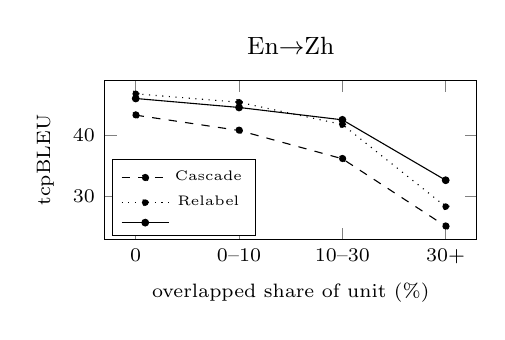
\begin{tikzpicture}\begin{axis}[width=0.52\columnwidth,height=3.6cm,xtick={0,1,2,3},
xticklabels={0,0--10,10--30,30+},xlabel={overlapped share of unit (\%)},ylabel={tcpBLEU},title={En$\rightarrow$Zh},
title style={font=\small},label style={font=\scriptsize},tick label style={font=\scriptsize},legend style={font=\tiny,at={(0.02,0.02)},anchor=south west}]
\addplot[dashed,mark=*,mark size=1.2pt] coordinates {(0,43.36) (1,40.84) (2,36.17) (3,25.04)}; \addlegendentry{Cascade}
\addplot[dotted,mark=*,mark size=1.2pt] coordinates {(0,46.88) (1,45.49) (2,41.82) (3,28.28)}; \addlegendentry{Relabel}
\addplot[solid,mark=*,mark size=1.2pt] coordinates {(0,46.11) (1,44.63) (2,42.59) (3,32.63)}; \addlegendentry{\sys{}}
\end{axis}\end{tikzpicture}
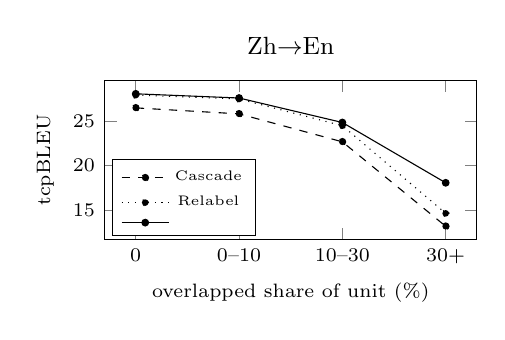
\begin{tikzpicture}\begin{axis}[width=0.52\columnwidth,height=3.6cm,xtick={0,1,2,3},
xticklabels={0,0--10,10--30,30+},xlabel={overlapped share of unit (\%)},ylabel={tcpBLEU},title={Zh$\rightarrow$En},
title style={font=\small},label style={font=\scriptsize},tick label style={font=\scriptsize},legend style={font=\tiny,at={(0.02,0.02)},anchor=south west}]
\addplot[dashed,mark=*,mark size=1.2pt] coordinates {(0,26.48) (1,25.81) (2,22.67) (3,13.19)}; \addlegendentry{Cascade}
\addplot[dotted,mark=*,mark size=1.2pt] coordinates {(0,27.91) (1,27.48) (2,24.48) (3,14.64)}; \addlegendentry{Relabel}
\addplot[solid,mark=*,mark size=1.2pt] coordinates {(0,28.06) (1,27.59) (2,24.84) (3,18.07)}; \addlegendentry{\sys{}}
\end{axis}\end{tikzpicture}
\caption{tcpBLEU by how much of a reference unit overlaps another speaker (reference windows, offline systems). The gap
between \sys{} and post-hoc relabelling opens where speakers overlap.}
\label{fig:overlap8}
\end{figure}


\paragraph{Labels or translation?} Relabelling \sys{}'s own output with the diarizer, keeping its text, separates the
two: on overlapped units its own labels score \num{v8:ov:en2zh:O2:ov} against
\num{v8:ov:en2zh:O2-relabel:ov} with diarizer labels (Zh$\rightarrow$En \num{v8:ov:zh2en:O2:ov} vs.\
\num{v8:ov:zh2en:O2-relabel:ov}), while with diarizer labels on both sides its text leads the speaker-blind model's by
\num{v8:ov:en2zh:O2-relabel:ov} vs.\ \num{v8:ov:en2zh:O2-nosd-relabel:ov}. Decoder-side speaker conditioning therefore mainly yields better
attributed segments under overlap: relabelling \sys{}'s own text costs \num{v8:ov:en2zh:O2:ov}$\rightarrow$\num{v8:ov:en2zh:O2-relabel:ov},
while its text with diarizer labels is only \num{v8:ov:en2zh:O2-relabel:ov} vs.\ \num{v8:ov:en2zh:O2-nosd-relabel:ov} for the
speaker-blind text; we do not claim that it translates overlapped speech better.

\paragraph{Short-turn fallback.} For every window, a cascade segment of at most 1.5\,s is added to \sys{}'s output
when no \sys{} segment of the same diarizer slot overlaps it within 0.5\,s and no nearby \sys{} text has chrF $\ge$50 with
it. On offline \sys{} this raises tcpBLEU in all three sets (Table~\ref{tab:overlap8}) and concurrent-speaker recall to
\num{v8:ov:en2zh:C2_O:cr} / \num{v8:ov:zh2en:C2_O:cr} / \num{v8:ov:ali:C2_O:cr}\%; on \sys{}-Simul it raises recall but
lowers tcpBLEU slightly, so by the criterion of the analysis plan it is adopted only for the offline model.

\paragraph{Latency.} Table~\ref{tab:lat8} queues the reads of a meeting on one decoder stream at the median single-stream
read time measured earlier (batch 1, two H200 cards, HuggingFace eager decoding). A wall-clock replay could only run beside another
job that held about \num{v8:b6:foreign_gib}\,GiB and most of the compute of every card,
with the Thinker spread over three cards at batch 1, so its real-time factor is an upper bound on the single-stream one.
On the one meeting completed (AliMeeting \num{v8:b6:ali_S2dl:meeting}, \sys{}-Simul) the median read took
\num{v8:b6:ali_S2dl:readp50}\,ms, \num{v8:b6:ali_S2dl:over}\% of the reads exceeded the 1\,s cadence, and the measured
real-time factor is \num{v8:b6:ali_S2dl:rtf}. By the rule of the analysis plan this is inconclusive, not a negative result:
contention only slows reads down, and an upper bound above 1 says nothing about the uncontended case. The remaining
replay runs were stopped, since further contended runs could not change that conclusion; two runs stopped part-way
(En$\rightarrow$Zh \sys{}-Simul, \num{v8:b6:en2zh_S2dl:done} of \num{v8:b6:en2zh_S2dl:of} windows; AliMeeting LocalAgreement,
\num{v8:b6:ali_O2_LA2:done} of \num{v8:b6:ali_O2_LA2:of}) are not used. The real-time factors of Table~\ref{tab:lat8} remain
estimates from the measured single-stream read time, not a replay.\ifWallclock{} A measured replay of the final systems is in Appendix~\ref{app:wallclock} (\sys{}'s Thinker does not keep up on AliMeeting).\fi{} LocalAgreement's reads take longer than the 1\,s read period, so queued it falls
behind without bound (per-speaker median \num{v8:lat:en2zh:O2_LA2:ps:p50}\,s). OpenSTBench-style start offset and
average delay of \sys{}-Simul (per-speaker channels, units spread uniformly over their block): \num{v8:lat:en2zh:S2dl:ps:start} and
\num{v8:lat:en2zh:S2dl:ps:atd}\,s in En$\rightarrow$Zh; these are not comparable with numbers reported on single-speaker
clips. Streams of more than 400 blocks (runaway repetition) were not synthesised: \num{v8:lat:ali:S2dl:ps:cens} on
AliMeeting, none elsewhere; counted as never heard, they leave the percentiles unchanged at the reported precision.

\paragraph{Fixed lag and seeds.} On an 8-meeting AMI subset (restricted for compute), fixed lag 2\,s on the
prefix-trained model scores \num{v8:sub:en2zh:lag2:all} tcpBLEU against \sys{}-Simul's \num{v8:sub:en2zh:on_S2dl:all} and
LocalAgreement's \num{v8:sub:en2zh:pla2:all} (En$\rightarrow$Zh; Zh$\rightarrow$En \num{v8:sub:zh2en:lag2:all} /
\num{v8:sub:zh2en:on_S2dl:all} / \num{v8:sub:zh2en:pla2:all}), but on overlapped units \num{v8:sub:en2zh:lag2:ov} vs.\
\num{v8:sub:en2zh:on_S2dl:ov} (\num{v8:sub:zh2en:lag2:ov} vs.\ \num{v8:sub:zh2en:on_S2dl:ov}), with a median text lag on
overlapped units of \num{v8:sub:en2zh:lag2:lagov} vs.\ \num{v8:sub:en2zh:on_S2dl:lagov}\,s. On the 10 AliMeeting subset
meetings (completed after the other runs, exploratory) fixed lag is ahead of \sys{}-Simul overall
and on overlapped units (\num{v8:sub:ali:lag2:all} / \num{v8:sub:ali:lag2:ov} vs.\ \num{v8:sub:ali:on_S2dl:all} /
\num{v8:sub:ali:on_S2dl:ov}; LocalAgreement \num{v8:sub:ali:pla2:all} / \num{v8:sub:ali:pla2:ov}), again at a longer lag on
overlapped units (\num{v8:sub:ali:lag2:lagov} vs.\ \num{v8:sub:ali:on_S2dl:lagov}\,s). Whole-meeting tcpBLEU of
\sys{}-Simul over training seeds: \num{v8:seed:en2zh:all} (En$\rightarrow$Zh, \num{v8:seed:en2zh:n} seeds; overlapped
\num{v8:seed:en2zh:ov}), \num{v8:seed:zh2en:all} (Zh$\rightarrow$En, \num{v8:seed:zh2en:n}), \num{v8:seed:ali:all}
(AliMeeting, \num{v8:seed:ali:n}).

\paragraph{Playback scheduling.} Table~\ref{tab:sched8} replays \sys{}-Simul's committed blocks under four single-channel
policies and the per-speaker layout. Captions for short overlapped interjections and skipping stale blocks bound the lag
of what is spoken, but on AliMeeting, where speakers overlap most, only \num{v8:b7:ali:d:cov}\% of the units are then
spoken.

\begin{table*}[t]
\centering\small
\begin{tabular}{lrrrrrrrrr}
\toprule
 & \multicolumn{3}{c}{En$\rightarrow$Zh} & \multicolumn{3}{c}{Zh$\rightarrow$En} & \multicolumn{3}{c}{AliMeeting} \\
\cmidrule(lr){2-4}\cmidrule(lr){5-7}\cmidrule(lr){8-10}
Playback & p50 & p90 & spoken & p50 & p90 & spoken & p50 & p90 & spoken \\
\midrule
one channel, as is & 142.4 & 772.6 & 100 & 26.4 & 313.0 & 100 & 604.6 & 2481.2 & 100 \\
short interjections as captions & 43.9 & 320.6 & 91 & 13.3 & 47.5 & 94 & 441.0 & 1630.3 & 93 \\
skip blocks $>$10\,s late & 9.7 & 11.8 & 80 & 9.8 & 13.1 & 82 & 10.8 & 17.2 & 35 \\
b + c & 9.1 & 11.6 & 80 & 9.4 & 12.9 & 82 & 10.8 & 17.4 & 35 \\
one channel per speaker, mixed & 7.4 & 12.2 & 100 & 8.2 & 15.1 & 100 & 23.2 & 314.1 & 100 \\
\bottomrule
\end{tabular}
\caption{Playback scheduling of \sys{}-Simul's whole-meeting output (reads queued; nothing re-synthesised, so the speech
of every played block is unchanged): listener completion lag (s) of the units played, and the share of units spoken
(\%; the rest are shown as captions). Policies fixed before any scheduling result.}
\label{tab:sched8}
\end{table*}


\paragraph{Voice prompts.} On 8 whole AMI En$\rightarrow$Zh meetings (3{,}318 output
streams), the Talker was run again with only the most recent 1\,s of a slot heard alone as its prompt instead of up to
8\,s, nothing else changed. The short prompt makes the voices less like the attributed speaker (WavLM SIM
\num{v8:b8:1s:sim} vs.\ \num{v8:b8:8s:sim}, meeting-bootstrap intervals \num{v8:b8:1s:simci} and \num{v8:b8:8s:simci}),
more often closer to another speaker of the window (\num{v8:b8:1s:conf} vs.\ \num{v8:b8:8s:conf}\%) and slightly less
intelligible (ASR-BLEU against the Talker's input \num{v8:b8:1s:asr} vs.\ \num{v8:b8:8s:asr}), so we keep 8\,s. At the
first commit \num{v8:b8:avail1}\% of the streams have 1\,s heard alone and \num{v8:b8:avail8}\% a full 8\,s. Holding a
slot's speech until 1\,s of it has been heard alone, instead of starting with the fallback prompt, would delay
\num{v8:b8:wait:streams}\% of the streams (\num{v8:b8:wait:blocks}\% of the blocks), but those by a median
\num{v8:b8:wait:p50}\,s (90th percentile \num{v8:b8:wait:p90}\,s): slots that rarely talk alone. Speaking at once is the
better default.

\paragraph{Threshold flips.} The causality check (Appendix~\ref{app:causal}) found \num{v8:b5:frames} distinct
80\,ms frames whose 0.5 activity decision differs between the prefix run and the dump. Rebuilding the online windows
with the prefix values changes \num{v8:b5:bound_same} window boundaries (none moves). The \num{v8:b5:windows} windows
holding a flipped frame were decoded again, each together with a copy using the original posteriors in the same batch:
\num{v8:b5:flip_same} are token-identical; an unchanged copy decoded in the same batch is identical in
\num{v8:b5:dup_same}. With so few windows the two cannot be told apart: the flips change outputs no more than
re-decoding does, but this check cannot show that they change nothing.

\paragraph{Full-coverage references.} The reference windows keep \num{v6:filt:en2zh:all:dur}\% of the En$\rightarrow$Zh
test speech. Every test utterance has a selected translation (Appendix~\ref{app:data}), so we also score the whole-meeting
runs on all \num{v8:full:en2zh:on_S2dl:units} non-hesitation units: \sys{}-Simul \num{v8:full:en2zh:on_S2dl:all}, LocalAgreement
on the offline model \num{v8:full:en2zh:on_O2_LA2:all}; overlapped units \num{v8:full:en2zh:on_S2dl:ov} vs.\
\num{v8:full:en2zh:on_O2_LA2:ov}. These are still machine translations.

